



Complex analysis has a strange quality to it -- results that are hard-won over the reals (and often false there!) come almost for free once we work over $\C$. A function that is complex differentiable once is differentiable infinitely often, is given locally by its Taylor series, and is essentially determined everywhere by its behaviour on a tiny region. This course is about what you can \emph{do} with all of that structure. We will use complex functions to map complicated regions onto simple ones (and solve Laplace's equation while doing so), evaluate real integrals that resist every technique of real calculus, and invert Fourier and Laplace transforms to solve differential equations.

This article constitutes my notes for the `Complex Methods' course, held in Lent 2021 at Cambridge. These notes are \emph{not a transcription of the lectures}, and differ significantly in quite a few areas. Still, all lectured material should be covered. These notes are also designed to complement my notes for the `Complex Analysis' course, which covers the same core theory but with an emphasis on rigour\footnote{The two courses share their central theorems -- Cauchy's theorem, Taylor and Laurent series, the residue theorem -- and lead to the same examination questions on that material. Where a careful proof exists in my Complex Analysis notes I will generally cite it rather than repeat it, and spend the space here on computations and applications instead.}. In this article we take the applied point of view: proofs are given when they are short or genuinely illuminating, and are otherwise sketched or omitted with a reference.



\section{Analytic Functions}

The star of this course is the \emph{analytic function} -- a complex function which is complex differentiable. This first section develops what that means, how to recognise such functions, and the surprisingly rigid structure that differentiability imposes. Already in this section we will meet the connection with Laplace's equation, which drives many of the physical applications later on.

\subsection{The Extended Complex Plane}

We will assume basic familiarity with the complex numbers themselves: every $z \in \C$ can be written as $z = x + iy$ with $x, y \in \R$, or in polar form as
$$
z = re^{i\theta} = r(\cos \theta + i \sin \theta),
$$
where $r = |z|$ and $\theta = \arg z$. The argument is only defined up to adding multiples of $2\pi$, a seemingly innocent remark that will cause us a surprising amount of grief in Section 2.

An `open set' will mean the same as it does in analysis: $D \subseteq \C$ is \vocab{open} if for every $z \in D$ there is some $\epsilon > 0$ such that the disc $\{w : |w - z| < \epsilon\}$ lies in $D$. A \vocab{domain} is a non-empty open set in which any two points can be joined by a path lying in the set. Domains are the natural habitat of the functions in this course.

It is frequently convenient to add a single `point at infinity' to the complex plane.

\begin{definition}[Extended Complex Plane]
	The \vocab{extended complex plane} is $\C^* = \C \cup \{\infty\}$, the complex plane together with a single extra point $\infty$.
\end{definition}

One can visualise $\C^*$ as a sphere (the \emph{Riemann sphere}): place a sphere on the plane, and join each point $z \in \C$ to the north pole by a straight line. That line meets the sphere at one other point, and this gives a bijection between $\C$ and the sphere minus the north pole. The north pole itself then corresponds to $\infty$. Points far from the origin in any direction are all close to the north pole, which is why a single point at infinity (rather than one for each direction, as one does with $\pm\infty$ in $\R$) is the natural choice.

To study the behaviour of a function $f$ `at infinity', we simply study $f(1/z)$ at $z = 0$. We will use this idea repeatedly, and it is worth internalising: \emph{infinity is not a special place, it just looks far away from where we are standing}.

\subsection{Complex Differentiation and the Cauchy--Riemann Equations}

We define differentiability exactly as we do over the reals.

\begin{definition}[Differentiability]
	A function $f : \C \to \C$ is \vocab{differentiable} at $z$ if the limit
	$$
	f'(z) = \lim_{\delta z \to 0} \frac{f(z + \delta z) - f(z)}{\delta z}
	$$
	exists.
\end{definition}

The definition looks identical to the real one, but it is far more demanding. The increment $\delta z$ is a complex number, and may approach $0$ from \emph{any direction} in the plane -- along the real axis, along the imaginary axis, along a spiral -- and the limit must be the same however it does so. This is a strong constraint, and it is what gives complex differentiable functions their remarkable properties.

\begin{definition}[Analytic Function]
	A function $f$ is \vocab{analytic}\footnote{The words \emph{holomorphic} and \emph{regular} are also used, particularly in the Complex Analysis course. In this course `analytic' is traditional.} at a point $z$ if it is differentiable throughout some open set containing $z$. A function analytic on all of $\C$ is called \vocab{entire}.
\end{definition}

Note the subtlety: analyticity at $z$ requires differentiability \emph{near} $z$, not just at $z$. This makes analyticity a much more robust notion, and it is the one we care about.

Let's extract something concrete from the definition. Write $z = x + iy$ and
$$
f(z) = u(x, y) + i v(x, y),
$$
where $u$ and $v$ are real-valued functions of two real variables. Suppose $f$ is differentiable at $z$. Then we may compute $f'(z)$ by letting $\delta z \to 0$ along whichever direction we please, and comparing the answers.

Taking $\delta z = \delta x$ real, we get
$$
f'(z) = \lim_{\delta x \to 0} \frac{f(z + \delta x) - f(z)}{\delta x} = \frac{\partial u}{\partial x} + i \frac{\partial v}{\partial x}.
$$
Taking $\delta z = i \, \delta y$ purely imaginary instead,
$$
f'(z) = \lim_{\delta y \to 0} \frac{f(z + i\delta y) - f(z)}{i \, \delta y} = \frac{1}{i}\left(\frac{\partial u}{\partial y} + i \frac{\partial v}{\partial y}\right) = \frac{\partial v}{\partial y} - i \frac{\partial u}{\partial y}.
$$
These must be equal, and comparing real and imaginary parts gives the fundamental equations of the subject.

\begin{theorem}[Cauchy--Riemann Equations]
	If $f = u + iv$ is differentiable at $z = x + iy$, then at that point
	$$
	\frac{\partial u}{\partial x} = \frac{\partial v}{\partial y}, \qquad \frac{\partial u}{\partial y} = -\frac{\partial v}{\partial x}.
	$$
\end{theorem}

The converse is almost true: it can fail if the partial derivatives exist but are badly discontinuous.

\begin{theorem}[Converse to Cauchy--Riemann]
	If $u$ and $v$ have continuous first-order partial derivatives satisfying the Cauchy--Riemann equations throughout an open set $D$, then $f = u + iv$ is analytic on $D$.
\end{theorem}
\begin{proof}[Proof (Sketch)]
	With continuous partials we can expand to first order:
	\begin{align*}
		\delta f &= u(x + \delta x, y + \delta y) - u(x, y) + i \big( v(x + \delta x, y + \delta y) - v(x, y)\big) \\
		&= \left(\frac{\partial u}{\partial x} + i \frac{\partial v}{\partial x}\right)\delta x + \left(\frac{\partial u}{\partial y} + i \frac{\partial v}{\partial y}\right)\delta y + o(|\delta z|).
	\end{align*}
	Applying the Cauchy--Riemann equations to the second bracket turns the right hand side into $\left(\frac{\partial u}{\partial x} + i \frac{\partial v}{\partial x}\right)(\delta x + i \delta y) + o(|\delta z|)$, so $\delta f/\delta z$ tends to a limit independent of the direction of $\delta z$.
\end{proof}

So, up to a regularity condition that never bites in practice, \emph{analytic = Cauchy--Riemann}. This gives us a practical test, and it's worth seeing it in action both on functions that pass and functions that fail.

\begin{example}[Analytic Functions]
	\begin{enumerate}[label=(\roman*)]
		\item Any polynomial in $z$ is entire -- sums, products and compositions of differentiable functions are differentiable, with the same proofs as in real analysis (the familiar product, quotient and chain rules all hold).
		\item The exponential
		$$
		e^z = e^x(\cos y + i \sin y)
		$$
		is entire, as one can check directly from the Cauchy--Riemann equations: $u = e^x \cos y$ and $v = e^x \sin y$ give $u_x = e^x \cos y = v_y$ and $u_y = -e^x \sin y = -v_x$. Differentiating, $\frac{\dd}{\dd z} e^z = u_x + i v_x = e^z$, as we'd hope.
		\item Any rational function $P(z)/Q(z)$ is analytic away from the zeros of $Q$. These `almost analytic' functions will be of great interest when we come to residue calculus -- the places where analyticity fails are exactly where the action is.
	\end{enumerate}
\end{example}

\begin{example}[Non-Analytic Functions]
	Consider $f(z) = \overline{z} = x - iy$, so $u = x$ and $v = -y$. Then $u_x = 1$ but $v_y = -1$, so the Cauchy--Riemann equations fail \emph{everywhere}, and $\overline{z}$ is nowhere differentiable, despite being a perfectly smooth function of $(x,y)$. Similarly $f(z) = |z|^2 = x^2 + y^2$ has $u_x = 2x$, $v_y = 0$, $u_y = 2y$, $v_x = 0$, so the equations hold only at $z = 0$. Thus $|z|^2$ is differentiable at the origin only, and analytic \emph{nowhere} -- there is no open set of differentiability.
\end{example}

The moral of these examples: a function is analytic when it is genuinely a function `of $z$ alone', and not of $\overline{z}$. This slogan can be made precise -- writing $x = (z + \overline z)/2$ and $y = (z - \overline z)/2i$, one can treat $z$ and $\overline{z}$ as independent variables, and then the Cauchy--Riemann equations become the single equation
$$
\frac{\partial f}{\partial \overline{z}} = 0.
$$

Before moving on, let's assemble the standard library of analytic functions, since we will compute with them constantly. Each is defined by the natural extension of its real Taylor series (or in terms of $e^z$), and each is entire:
\begin{align*}
	\sin z = \frac{e^{iz} - e^{-iz}}{2i}, &\qquad \cos z = \frac{e^{iz} + e^{-iz}}{2}, \\
	\sinh z = \frac{e^{z} - e^{-z}}{2}, &\qquad \cosh z = \frac{e^{z} + e^{-z}}{2}.
\end{align*}
Over $\C$, the trigonometric and hyperbolic families merge into one: from the definitions,
$$
\sin(iz) = i \sinh z, \qquad \cos(iz) = \cosh z,
$$
and all the usual addition formulas hold verbatim (they are identities between analytic functions that agree on $\R$ -- and, as is shown in Complex Analysis, analytic functions agreeing on a line agree everywhere). Some facts worth internalising now, as they shape all the contour arguments to come:

\begin{enumerate}[label=(\roman*)]
	\item $e^z$ is periodic with period $2\pi i$, and is \emph{never zero}: $|e^z| = e^x > 0$.
	\item $\sin z$ and $\cos z$ are \emph{unbounded} off the real axis -- e.g.\ $\cos(iy) = \cosh y \to \infty$. Boundedness of $\sin$ and $\cos$ is a purely real-variable accident.
	\item The zeros of $\sin z$ and $\cos z$ are exactly the familiar real ones, $n\pi$ and $(n + \frac 12)\pi$. Writing $\sin(x + iy) = \sin x \cosh y + i \cos x \sinh y$, both terms vanish only when $y = 0$ and $\sin x = 0$.
	\item Correspondingly $\sinh z$ has zeros exactly at $z = n\pi i$, and $\cosh z$ at $z = \left(n + \frac 12\right)\pi i$ -- on the \emph{imaginary} axis. These lattices of zeros will reappear as lattices of poles of $1/\cosh$ and friends in Section 6.
\end{enumerate}

For working in polar coordinates -- which we will do constantly once branch cuts appear -- it is useful to have the polar form of the Cauchy--Riemann equations.

\begin{proposition}[Cauchy--Riemann in Polar Form]
	Let $f(z) = u(r, \theta) + iv(r, \theta)$ where $z = re^{i\theta}$. Then the Cauchy--Riemann equations take the form
	$$
	\frac{\partial u}{\partial r} = \frac{1}{r}\frac{\partial v}{\partial \theta}, \qquad
	\frac{\partial v}{\partial r} = -\frac{1}{r} \frac{\partial u}{\partial \theta},
	$$
	and then $f'(z) = e^{-i\theta}\left(u_r + i v_r\right)$.
\end{proposition}
\begin{proof}
	This is a chain rule computation. From $x = r \cos\theta$, $y = r\sin \theta$ we get
	$$
	\frac{\partial u}{\partial r} = u_x \cos \theta + u_y \sin \theta, \qquad \frac{\partial u}{\partial \theta} = -u_x r \sin\theta + u_y r \cos\theta,
	$$
	and similarly for $v$. Substituting the Cartesian Cauchy--Riemann equations $u_x = v_y$, $u_y = -v_x$ into these expressions gives
	$$
	\frac{1}{r} \frac{\partial v}{\partial \theta} = -v_x \sin \theta + v_y \cos\theta = u_y \sin\theta + u_x \cos\theta = \frac{\partial u}{\partial r},
	$$
	and the second equation follows in the same way. For the derivative, approach along a ray of constant $\theta$, so $\delta z = e^{i\theta} \, \delta r$, giving $f'(z) = e^{-i\theta}(u_r + iv_r)$.
\end{proof}

\begin{example}[Powers and Logarithms]
	Take $f(z) = z^c$ for a real constant $c$, defined (for now, for $r>0$ and some range of $\theta$) by $f = r^c e^{ic\theta}$, so $u = r^c \cos c\theta$ and $v = r^c \sin c\theta$. Then
	$$
	u_r = cr^{c-1}\cos c\theta = \frac{1}{r} v_\theta, \qquad v_r = c r^{c - 1} \sin c\theta = -\frac{1}{r} u_\theta,
	$$
	so $z^c$ is analytic where defined, with
	$$
	f'(z) = e^{-i\theta} \cdot c r^{c-1} e^{i c \theta} = c z^{c - 1}.
	$$
	An identical computation shows $\log z = \log r + i\theta$ satisfies the polar Cauchy--Riemann equations with $\frac{\dd}{\dd z} \log z = e^{-i\theta} \cdot \frac{1}{r} = \frac{1}{z}$. The phrase `where defined' is hiding real content here -- pinning down where these functions can be defined is the subject of Section 2.
\end{example}

\subsection{Harmonic Functions}

We now come to the first connection with applied mathematics, and it is a spectacular one. Recall Laplace's equation for a function $\phi(x, y)$:
$$
\nabla^2 \phi = \frac{\partial^2 \phi}{\partial x^2} + \frac{\partial^2 \phi}{\partial y^2} = 0.
$$
This is arguably the most important partial differential equation there is: it governs steady-state temperature distributions, electrostatic potentials, gravitational potentials, and the flow of ideal fluids.

\begin{definition}[Harmonic Function]
	A function $\phi : \R^2 \to \R$ satisfying $\nabla^2 \phi = 0$ is \vocab{harmonic}.
\end{definition}

Here is the connection.

\begin{proposition}
	If $f = u + iv$ is analytic on a domain $D$, then $u$ and $v$ are both harmonic on $D$.
\end{proposition}
\begin{proof}
	We use the fact (immediate from results in Complex Analysis, where it is shown that analytic functions are infinitely differentiable) that $u$ and $v$ have continuous second derivatives. Then, using the Cauchy--Riemann equations twice,
	$$
	\frac{\partial^2 u}{\partial x^2} = \frac{\partial}{\partial x}\frac{\partial v}{\partial y} = \frac{\partial}{\partial y} \frac{\partial v}{\partial x} = \frac{\partial}{\partial y}\left(-\frac{\partial u}{\partial y}\right) = -\frac{\partial^2 u}{\partial y^2},
	$$
	so $u$ is harmonic, and likewise for $v$.
\end{proof}

So the real and imaginary parts of \emph{any} analytic function hand us solutions of Laplace's equation, entirely for free. The functions $u$ and $v$ obtained in this way are not unrelated, and we give the relationship a name.

\begin{definition}[Harmonic Conjugate]
	Two harmonic functions $u$ and $v$ satisfying the Cauchy--Riemann equations are \vocab{harmonic conjugates}, and then $u + iv$ is analytic.
\end{definition}

Given a harmonic function $u$, we can reconstruct its harmonic conjugate (up to a constant) directly from the Cauchy--Riemann equations, by integrating one equation and differentiating the result. This is best seen by example.

\begin{example}[Finding a Harmonic Conjugate]
	Let $u(x, y) = x^2 - y^2$, which is easily checked to be harmonic. We seek $v$ with
	$$
	\frac{\partial v}{\partial y} = \frac{\partial u}{\partial x} = 2x
	\quad \implies \quad
	v = 2xy + g(x)
	$$
	for some function $g$ of $x$ alone. The other Cauchy--Riemann equation demands
	$$
	\frac{\partial v}{\partial x} = 2y + g'(x) = -\frac{\partial u}{\partial y} = 2y,
	$$
	so $g$ is a constant, and $v = 2xy + c$. Sure enough,
	$$
	u + iv = x^2 - y^2 + 2ixy + ic = z^2 + ic,
	$$
	and we have recognised our harmonic function as the real part of an analytic one.
\end{example}

One caution about existence. The construction above is local -- it works on any disc -- but on domains with holes, a harmonic function need not have a \emph{single-valued} conjugate globally. The standard example is $u = \log|z|$ on the punctured plane: its conjugate wants to be $\theta = \arg z$, which (as Section 2 will make much of) cannot be defined continuously all the way around the origin. On simply connected domains this problem never arises, and every harmonic function is globally the real part of an analytic one.

\begin{example}[A Conjugate in Polar Coordinates]
	Let $u = r^2 \cos 2\theta$ (which is $\re z^2$ in disguise, but let's pretend we don't know that). The polar Cauchy--Riemann equations give
	$$
	\frac{\partial v}{\partial \theta} = r \frac{\partial u}{\partial r} = 2r^2 \cos 2\theta
	\quad\implies\quad
	v = r^2 \sin 2\theta + g(r),
	$$
	and then $\frac{\partial v}{\partial r} = 2r \sin 2\theta + g'(r)$ must equal $-\frac 1r u_\theta = 2r \sin 2\theta$, so $g$ is constant. Thus $v = r^2 \sin 2\theta + c$ and $u + iv = r^2 e^{2i\theta} + ic = z^2 + ic$, as expected.
\end{example}

The level curves of $u$ and $v$ carry geometric information too. If $f = u + iv$ is analytic, then
$$
\nabla u \cdot \nabla v = u_x v_x + u_y v_y = -u_x u_y + u_y u_x = 0,
$$
using the Cauchy--Riemann equations. So \emph{the level curves of $u$ and $v$ are orthogonal} wherever $f' \neq 0$. If $u$ is an electrostatic potential, the curves $u = \text{const}$ are equipotentials and the curves $v = \text{const}$ are field lines; if $v$ is the stream function of a fluid flow, the curves $v = \text{const}$ are streamlines and $u$ is the velocity potential. One analytic function packages the whole picture. We will exploit this systematically in Section 3.

Let's record the fluid dynamics dictionary now, as we will want it later.

\begin{remark}[Complex Potentials for Fluid Flow]
	For steady, incompressible, irrotational flow in the plane with velocity $(u_1, u_2)$, there is a velocity potential $\phi$ (with $\nabla \phi = (u_1, u_2)$, existing since the flow is irrotational) and a stream function $\psi$ (existing since the flow is incompressible), and both are harmonic. The \vocab{complex potential} is the analytic function
	$$
	w(z) = \phi + i \psi,
	$$
	and the velocity is recovered from $w'(z) = u_1 - i u_2$. The flow is along the level curves of $\psi$. For example, $w(z) = Uz$ is uniform flow with speed $U$ in the $x$-direction, and $w(z) = U(z + a^2/z)$ will turn out to describe flow past a circular cylinder of radius $a$.
\end{remark}

\section{Multivalued Functions and Branch Cuts}

We have already brushed against the problem twice: both $\log z$ and $z^c$ were only defined once we chose a range for $\theta = \arg z$. This section confronts the issue properly. It is a genuinely subtle business -- more subtle than it first appears -- and it matters a great deal in practice, since the placement of branch cuts is exactly what makes certain real integrals computable in Section 6.

\subsection{The Problem with the Logarithm}

For $z = re^{i\theta} \neq 0$ we would like to define
$$
\log z = \log r + i\theta.
$$
But $\theta$ is only defined up to multiples of $2\pi$, so this definition assigns infinitely many values to each point:
$$
\log i = \frac{\pi i}{2} \;\text{ or }\; \frac{5\pi i}{2} \;\text{ or }\; -\frac{3\pi i}{2} \;\text{ or } \cdots.
$$
We say $\log$ is a \vocab{multivalued function}. One might hope to fix this by just picking a value at each point -- say, always take $\theta \in (0, 2\pi]$. But an arbitrary choice like this creates discontinuities, and where those discontinuities can and cannot go is the heart of the matter.

Consider tracking a value of $\log z$ continuously along each of the following three curves.

\begin{center}
\begin{tikzpicture}[scale=0.9]
	\draw[->] (-3, 0) -- (3, 0);
	\draw[->] (0, -2.6) -- (0, 2.6);
	\draw[blue, thick, ->-=0.25] (2.85, 1.1) arc(0:360:0.5);
	\node[blue] at (2.35, 1.85) {$C_1$};
	\draw[blue, thick, ->-=0.25] (-1.5, -1.1) arc(0:360:0.5);
	\node[blue] at (-2, -2.15) {$C_2$};
	\draw[blue, thick, ->-=0.12] (1.6, 0) arc(0:360:1.6);
	\node[blue] at (1.5, -1.55) {$C_3$};
	\fill (0,0) circle (0.05);
\end{tikzpicture}
\end{center}

On $C_1$, which stays in the right half-plane, we can fix $\theta \in (-\frac{\pi}{2}, \frac{\pi}{2})$ throughout, and $\log z$ is continuous and single-valued all the way round. On $C_2$ we can similarly fix a range of $\theta$ and all is well. But on $C_3$, which encircles the origin, there is no possible choice: following the curve anticlockwise once, $\theta$ must increase continuously by $2\pi$, so when we return to our starting point the value of $\log z$ has increased by $2\pi i$. The function must either jump somewhere on $C_3$, or fail to be single-valued. The origin is the source of the problem, and we give such points a name.

\begin{definition}[Branch Point]
	A \vocab{branch point} of a function is a point which it is impossible to encircle with a closed curve on which the function is both continuous and single-valued. The function is said to have a \vocab{branch point singularity} there.
\end{definition}

\begin{example}[Spotting Branch Points]
	\begin{enumerate}[label=(\roman*)]
		\item $\log(z - a)$ has a branch point at $z = a$.
		\item $z^c = r^c e^{ic\theta}$ has a branch point at the origin whenever $c \notin \Z$: going once anticlockwise around a circle of radius $r_0$, continuity forces the value to move from $r_0^c$ to $r_0^c e^{2\pi i c}$, and these differ unless $c$ is an integer.
		\item $\log z$ also has a branch point \emph{at infinity}: setting $\zeta = 1/z$, we get $\log z = -\log \zeta$, which has a branch point at $\zeta = 0$. Similarly $z^c$ has a branch point at infinity for $c \notin \Z$.
		\item $\displaystyle f(z) = \log\left(\frac{z - 1}{z + 1}\right) = \log(z-1) - \log(z+1)$ has branch points at $\pm 1$, but \emph{not} at infinity: with $\zeta = 1/z$ we get $\log\left(\frac{1 - \zeta}{1 + \zeta}\right)$, and for $\zeta$ near $0$ the quantity $\frac{1-\zeta}{1+\zeta}$ stays near $1$, well away from the troublesome points of $\log$. So small circles about $\zeta = 0$ cause no jump. (Equivalently: a giant circle in the $z$-plane winds around \emph{both} branch points, and the two jumps of $\pm 2\pi i$ cancel.)
	\end{enumerate}
\end{example}

\subsection{Branch Cuts}

Since the trouble comes from curves that wind around branch points, the remedy is blunt but effective: forbid them.

\begin{definition}[Branch Cut]
	A \vocab{branch cut} is a curve in the plane, joining branch points (or running from a branch point to infinity), which curves are forbidden from crossing. On the cut plane we can then make a consistent choice of value of the function; such a choice is called a \vocab{branch}, and it is single-valued and continuous on any curve avoiding the cut.
\end{definition}

For $\log z$, the standard choice is to cut along the negative real axis, and take $\theta \in (-\pi, \pi]$:

\begin{center}
\begin{tikzpicture}[scale=0.9]
	\draw[->] (-2.8, 0) -- (2.8, 0);
	\draw[->] (0, -1.3) -- (0, 2.2);
	\draw[thick, decorate, decoration={zigzag, segment length=5pt, amplitude=1.2pt}] (-2.8, 0) -- (0, 0);
	\fill (0,0) circle (0.05);
	\draw (0, 0) -- (1.9, 1.25) node[circle, fill, inner sep = 1pt] {} node[right] {$z$};
	\draw (0.55, 0) arc (0:33.3:0.55);
	\node at (0.82, 0.28) {$\theta$};
\end{tikzpicture}
\end{center}

This is called the \vocab{principal branch} of the logarithm, and its value the \vocab{principal value}. The principal branch is analytic on the cut plane, with $\frac{\dd}{\dd z}\log z = \frac{1}{z}$, but on the cut itself it is not even continuous: just above the cut at $z = x + i0^+$ (with $x < 0$) we have $\log z = \log|x| + i\pi$, while just below at $z = x + i0^-$ we have $\log z = \log |x| - i\pi$. The function jumps by $2\pi i$ across the cut. This jump is not a defect -- in Section 6 it will be precisely the tool that lets us evaluate integrals.

Some remarks on the choices being made here:
\begin{enumerate}[label=(\roman*)]
	\item The cut itself is a choice. Any curve from $0$ to $\infty$ works -- the non-negative imaginary axis (with, say, $\theta \in (-\frac{3\pi}{2}, \frac{\pi}{2}]$), or even a wiggly curve. All that matters is that curves can no longer wind around the branch point.
	\item Even after fixing the cut, the branch is a further choice: with the cut on the negative real axis we could take $\theta \in (\pi, 3\pi]$ instead, which changes $\log z$ by $2\pi i$ everywhere.
	\item In any problem where a branch matters, you must specify it -- either by giving the range of $\theta$ explicitly, or by giving the location of the cut together with the value of the branch at one point (the values everywhere else are then pinned down by continuity).
\end{enumerate}

The same considerations apply verbatim to $z^c$ for $c \notin \Z$, whose branches on the cut plane are $r^c e^{ic\theta}$ with $\theta$ in a chosen range of length $2\pi$. Note the different branches of $z^c$ differ by constant factors $e^{2\pi i c k}$, and for $z^{1/2}$ there are exactly two branches, differing by a sign -- just as we would expect for a square root.

\begin{remark}[Riemann Surfaces]
	There is a more elegant point of view, due to Riemann: rather than forbidding curves from crossing the cut, imagine infinitely many copies of the cut plane stacked above one another, with the top edge of each cut glued to the bottom edge of the cut on the next sheet up. Crossing the cut moves you to the adjacent sheet, where $\log z$ takes its next branch's values. On this spiral staircase -- the \emph{Riemann surface} of $\log$ -- the logarithm is a perfectly ordinary single-valued analytic function. Riemann surfaces get an entire Part II course, and we say no more about them here.
\end{remark}

\subsection{Multiple Branch Cuts}

When a function has several branch points, we may need several cuts, and there is some genuine artistry in choosing them well.

\begin{example}[Two Cuts to Infinity]
	Consider $f(z) = (z(z-1))^{1/3}$, with branch points at $0$ and $1$ (and at $\infty$). One valid choice is to cut from $0$ out to $-\infty$ along the real axis, and from $1$ out to $+\infty$:
	\begin{center}
	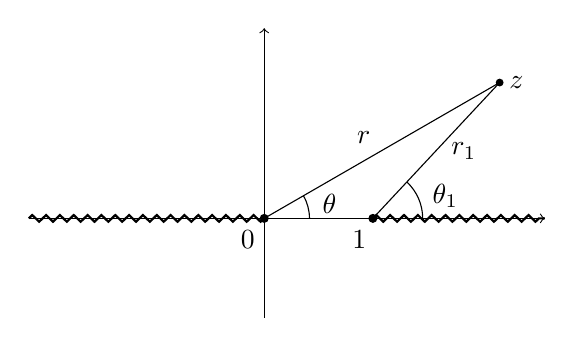
\begin{tikzpicture}[scale=1.15]
		\draw[->] (-2.6, 0) -- (3.1, 0);
		\draw[->] (0, -1.1) -- (0, 2.1);
		\draw[thick, decorate, decoration={zigzag, segment length=5pt, amplitude=1.2pt}] (-2.6, 0) -- (0, 0);
		\draw[thick, decorate, decoration={zigzag, segment length=5pt, amplitude=1.2pt}] (1.2, 0) -- (3.1, 0);
		\fill (0,0) circle (0.05);
		\fill (1.2,0) circle (0.05);
		\node[below] at (-0.18, -0.03) {$0$};
		\node[below] at (1.05, -0.03) {$1$};
		\draw (0, 0) -- (2.6, 1.5) node[circle, fill, inner sep=1pt] {} node[right] {$z$};
		\node[above] at (1.1, 0.72) {$r$};
		\draw (1.2, 0) -- (2.6, 1.5);
		\node[below right, inner sep=2pt] at (2.0, 0.9) {$r_1$};
		\draw (0.5, 0) arc (0:30:0.5);
		\node at (0.72, 0.16) {$\theta$};
		\draw (1.75, 0) arc (0:47:0.55);
		\node at (2.0, 0.25) {$\theta_1$};
	\end{tikzpicture}
	\end{center}
	Writing $z = re^{i\theta}$ with $\theta \in (-\pi, \pi]$ and $z - 1 = r_1 e^{i\theta_1}$ with $\theta_1 \in [0, 2\pi)$, we define
	$$
	f(z) = \sqrt[3]{r r_1} \, e^{i(\theta + \theta_1)/3}.
	$$
	Crossing either cut makes one of the angles jump, so $f$ jumps -- but away from the cuts, $f$ is continuous and single-valued, as no curve can now encircle either branch point alone.
\end{example}

However, sometimes we can get away with less. If a function has \emph{no} branch point at infinity, then large curves winding around all the finite branch points are harmless -- so we shouldn't waste a cut ruling them out.

\begin{example}[A Finite Cut]
	Take again
	$$
	f(z) = \log\left(\frac{z - 1}{z + 1}\right),
	$$
	with branch points at $\pm 1$ but not at $\infty$. Here we may take a single finite cut along the segment $[-1, 1]$:
	\begin{center}
	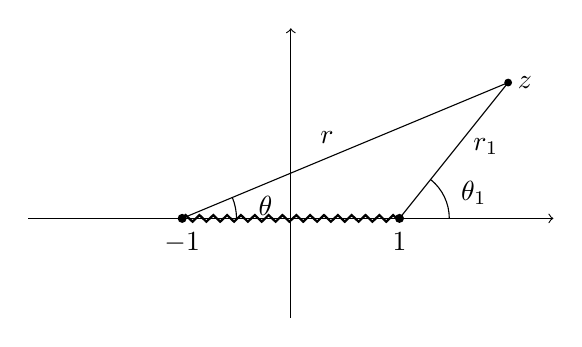
\begin{tikzpicture}[scale=1.15]
		\draw[->] (-2.9, 0) -- (2.9, 0);
		\draw[->] (0, -1.1) -- (0, 2.1);
		\draw[thick, decorate, decoration={zigzag, segment length=5pt, amplitude=1.2pt}] (-1.2, 0) -- (1.2, 0);
		\fill (-1.2,0) circle (0.05);
		\fill (1.2,0) circle (0.05);
		\node[below] at (-1.2, -0.05) {$-1$};
		\node[below] at (1.2, -0.05) {$1$};
		\draw (-1.2, 0) -- (2.4, 1.5) node[circle, fill, inner sep=1pt] {} node[right] {$z$};
		\node[above] at (0.4, 0.72) {$r$};
		\draw (1.2, 0) -- (2.4, 1.5);
		\node[below right, inner sep=2pt] at (1.95, 0.95) {$r_1$};
		\draw (-0.6, 0) arc (0:22.6:0.6);
		\node at (-0.28, 0.14) {$\theta$};
		\draw (1.75, 0) arc (0:51:0.55);
		\node at (2.02, 0.28) {$\theta_1$};
	\end{tikzpicture}
	\end{center}
	Write $z + 1 = re^{i\theta}$ and $z - 1 = r_1 e^{i\theta_1}$, and -- this is the part requiring thought -- take \emph{both} $\theta, \theta_1 \in [0, 2\pi)$. Then define
	$$
	f(z) = \log(r_1/r) + i(\theta_1 - \theta).
	$$
	Let's check this is continuous away from the cut. Crossing the real axis to the \emph{left} of the cut ($x < -1$): both $\theta$ and $\theta_1$ pass smoothly through $\pi$, so nothing happens. Crossing to the \emph{right} of the cut ($x > 1$): both $\theta$ and $\theta_1$ jump by $2\pi$ -- but $f$ depends only on the difference $\theta_1 - \theta$, so it doesn't notice. Crossing the cut itself ($-1 < x < 1$): $\theta_1$ jumps by $2\pi$ while $\theta$ varies smoothly, so $f$ jumps by $2\pi i$, exactly as a branch cut should.
\end{example}

This example is worth understanding well -- finite branch cuts of this type appear frequently on example sheets and in applications, and choosing the angle ranges correctly is the whole game. Let's do one more of the same flavour, since the square-root version is the one that appears most often.

\begin{example}[Branches of {$\sqrt{z^2 - 1}$}]
	The function $f(z) = (z^2 - 1)^{1/2} = ((z-1)(z+1))^{1/2}$ has branch points at $\pm 1$. Is there a branch point at infinity? With $\zeta = 1/z$,
	$$
	f = \frac{1}{\zeta}(1 - \zeta^2)^{1/2},
	$$
	and $(1 - \zeta^2)^{1/2}$ is single-valued near $\zeta = 0$ (the argument stays near 1) -- so no: for large $|z|$, $f(z) \approx \pm z$ consistently. We may therefore use a single finite cut along $[-1, 1]$.

	Write $z - 1 = r_1 e^{i\theta_1}$ and $z + 1 = r_2 e^{i\theta_2}$ with $\theta_1, \theta_2 \in [0, 2\pi)$, and set
	$$
	f(z) = \sqrt{r_1 r_2} \, e^{i(\theta_1 + \theta_2)/2}.
	$$
	Crossing the real axis to the right of the cut, both angles jump by $2\pi$, so $(\theta_1 + \theta_2)/2$ jumps by $2\pi$ -- invisible in the exponential. Crossing to the left of the cut, both angles pass smoothly through $\pi$. Crossing the cut itself, only $\theta_2$ jumps, so $f$ changes sign: a genuine discontinuity, as expected. On the top of the cut ($z = x$ with $-1 < x < 1$, approached from above) we have $\theta_1 = \pi$, $\theta_2 = 0$, so $f = i\sqrt{1 - x^2}$; on the bottom, $f = -i\sqrt{1 - x^2}$. For large real $z = x > 1$ we get $f = \sqrt{x^2 - 1} > 0$, so this branch behaves like $+z$ at infinity.

	Functions of exactly this type appear when one inverts Joukowski-type maps ($w = \frac 12 (z + \frac 1z)$ gives $z = w + \sqrt{w^2 - 1}$), and the cut along $[-1, 1]$ is the image of the unit circle -- the two branches correspond to the inside and outside of the circle.
\end{example}

A final practical point: a branch is often specified not by angle ranges but by its \emph{value at one point}, and one must then be able to evaluate it elsewhere by continuity. With the branch of $\sqrt{z^2 - 1}$ above (cut $[-1,1]$, $f(2) = +\sqrt 3$), what is $f(-2)$? Reading off the angles at $z = -2$: $\theta_1 = \theta_2 = \pi$, so $f(-2) = \sqrt{1 \cdot 3}\, e^{i(\pi + \pi)/2} = -\sqrt 3$. Note this is \emph{not} `$+\sqrt{(-2)^2 - 1}$' -- a single consistent branch of $\sqrt{z^2 - 1}$ must behave like $+z$ at one end of the real axis and hence like $z$ (i.e.\ negatively) at the other. Blindly taking positive square roots on both ends describes \emph{two different branches}, and is the single most common branch-cut error.

\section{Conformal Maps}

Here is the plan for this section. Laplace's equation is easy to solve on nice domains (half-planes, discs, strips) and hard to solve on nasty ones. Analytic functions, viewed as maps from one region of the plane to another, turn out to preserve exactly the structure Laplace's equation cares about. So if we can map our nasty domain onto a nice one by an analytic bijection, we can solve our problem on the nice domain and pull the solution back. This section builds up a toolkit of such maps, and then puts them to work.

\subsection{M\"obius Maps}

We begin with a class of maps you have met before, in IA Groups.

\begin{definition}[M\"obius Map]
	A \vocab{M\"obius map} is a map of the form
	$$
	z \mapsto w = \frac{az + b}{cz + d},
	$$
	where $a, b, c, d \in \C$ and $ad - bc \neq 0$.
\end{definition}

The condition $ad - bc \neq 0$ rules out the degenerate case where the map is constant. A M\"obius map is analytic everywhere except at $z = -d/c$, where the denominator vanishes. The right way to think about this is as a map of the \emph{extended} complex plane: setting
$$
-\frac{d}{c} \mapsto \infty, \qquad \infty \mapsto \frac{a}{c},
$$
a M\"obius map becomes a bijection $\C^* \to \C^*$, with inverse
$$
w \mapsto \frac{-dw + b}{cw - a},
$$
which is another M\"obius map. Composites of M\"obius maps are also M\"obius maps -- indeed they form a group under composition.

For our purposes their key property concerns circles and lines. It is convenient to treat these uniformly: a line is simply a circle through $\infty$.

\begin{definition}[Circline]
	A \vocab{circline} is a circle or a straight line.
\end{definition}

\begin{proposition}
	M\"obius maps send circlines to circlines.
\end{proposition}
\begin{proof}
	Every circline can be written as a circle of Apollonius
	$$
	|z - z_1| = \lambda|z - z_2|
	$$
	for some $z_1, z_2 \in \C$ and $\lambda > 0$, with $\lambda = 1$ giving lines and $\lambda \neq 1$ circles (this was on the first IA Vectors and Matrices example sheet). Substituting $z = \frac{-dw+b}{cw - a}$ and clearing denominators, this becomes
	$$
	|(cz_1 + d)w - (az_1 + b)| = \lambda |(cz_2 + d)w - (az_2 + b)|.
	$$
	If $cz_1 + d$ and $cz_2 + d$ are both non-zero, dividing through puts this in Apollonius form again, so the image is a circline; if one of them vanishes the equation directly describes a circle (or line).
\end{proof}

Note carefully what is \emph{not} claimed: circles may map to lines and vice versa. A circle passing through the point sent to $\infty$ must map to a line.

\begin{proposition}[Three-Point Determination]
	Given distinct points $\alpha, \beta, \gamma \in \C^*$ and distinct $\alpha', \beta', \gamma' \in \C^*$, there is a M\"obius map sending $\alpha \mapsto \alpha'$, $\beta \mapsto \beta'$, $\gamma \mapsto \gamma'$.
\end{proposition}
\begin{proof}
	The map
	$$
	f_1(z) = \frac{\beta - \gamma}{\beta - \alpha} \cdot \frac{z - \alpha}{z - \gamma}
	$$
	sends $\alpha \mapsto 0$, $\beta \mapsto 1$, $\gamma \mapsto \infty$. Building $f_2$ in the same way from the primed points, the composition $f_2^{-1} \circ f_1$ does the job (and is M\"obius, since M\"obius maps form a group).
\end{proof}

Since three points determine a circline, this means we can find a M\"obius map taking any circline to any other -- and hence, with a little care about which side is which, taking any disc or half-plane to any other disc or half-plane. This is exactly the flexibility we will want.

\subsection{Conformal Maps}

\begin{definition}[Conformal Map]
	A \vocab{conformal map} $f : U \to V$, where $U, V$ are open subsets of $\C$, is an analytic map with $f'(z) \neq 0$ for all $z \in U$. If additionally $f$ is a bijection $U \to V$, we call it a \vocab{conformal equivalence}.
\end{definition}

The name comes from the following geometric property.

\begin{proposition}[Conformal Maps Preserve Angles]
	A conformal map preserves the angle -- in both magnitude and orientation -- between intersecting curves.
\end{proposition}
\begin{proof}
	Let $z_1(t)$ be a curve passing through $z_0 = z_1(t_1)$ with non-zero tangent $z_1'(t_1)$, making angle $\phi = \arg z_1'(t_1)$ with the real axis. The image curve $Z_1(t) = f(z_1(t))$ has tangent
	$$
	Z_1'(t_1) = f'(z_0) \, z_1'(t_1),
	$$
	which makes angle $\arg f'(z_0) + \phi$ with the real axis (using $f'(z_0) \neq 0$ so its argument makes sense). So \emph{every} curve through $z_0$ has its tangent direction rotated by the same angle $\arg f'(z_0)$, and hence angles between pairs of curves are preserved.
\end{proof}

In fact the converse holds too (an angle-preserving map is conformal), though we won't prove it. Do note where the proof uses $f' \neq 0$: at a point where $f'$ vanishes, angles are genuinely \emph{not} preserved -- we will see in a moment that $z \mapsto z^2$ doubles angles at the origin.

When computing with conformal maps, the following procedure for finding the image $f(U)$ is invaluable: \emph{find the image of the boundary $\partial U$, which will be the boundary of $V$; then take any single convenient point of $U$ and see which side of that boundary its image lands on.}

\subsection{A Catalogue of Conformal Maps}

In practice one builds complicated conformal maps by composing simple standard ones (compositions of conformal maps are conformal, by the chain rule). Here is the standard toolkit.

\textbf{(i) Linear maps.} $z \mapsto az + b$ with $a \neq 0$ rotates by $\arg a$, scales by $|a|$, and translates by $b$. Conformal everywhere.

\textbf{(ii) Powers.} $z \mapsto z^\alpha$ (with a suitable branch when $\alpha \notin \Z$) is conformal away from the origin, and maps the sector $0 < \arg z < \phi$ to the sector $0 < \arg w < \alpha\phi$: it \emph{multiplies angles at the origin by $\alpha$}. For instance, $z \mapsto z^2$ maps the quarter-disc to the half-disc:
$$
U = \left\{z : |z| < 1, \ 0 < \arg z < \tfrac{\pi}{2}\right\} \quad \longrightarrow \quad V = \{w : |w| < 1, \ 0 < \arg w < \pi\}.
$$
\begin{center}
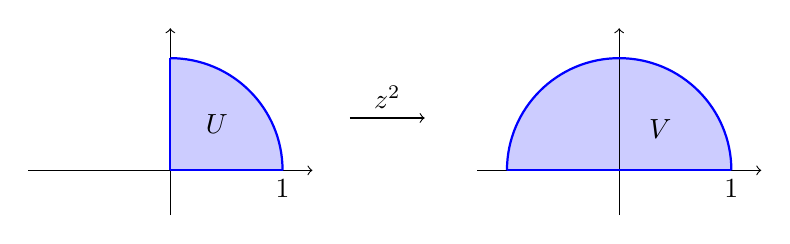
\begin{tikzpicture}[scale=0.95]
	\fill[blue!20] (0,0) -- (1.5, 0) arc (0:90:1.5) -- cycle;
	\draw[->] (-1.9, 0) -- (1.9, 0);
	\draw[->] (0, -0.6) -- (0, 1.9);
	\draw[blue, thick] (1.5, 0) arc (0:90:1.5);
	\draw[blue, thick] (0,0) -- (1.5,0);
	\draw[blue, thick] (0,0) -- (0,1.5);
	\node[below] at (1.5, 0) {$1$};
	\node at (0.62, 0.62) {$U$};
	\draw[->] (2.4, 0.7) -- (3.4, 0.7) node[pos=0.5, above] {$z^2$};
	\begin{scope}[shift={(6,0)}]
		\fill[blue!20] (-1.5, 0) -- (1.5, 0) arc (0:180:1.5) -- cycle;
		\draw[->] (-1.9, 0) -- (1.9, 0);
		\draw[->] (0, -0.6) -- (0, 1.9);
		\draw[blue, thick] (1.5, 0) arc (0:180:1.5);
		\draw[blue, thick] (-1.5,0) -- (1.5,0);
		\node[below] at (1.5, 0) {$1$};
		\node at (0.55, 0.55) {$V$};
	\end{scope}
\end{tikzpicture}
\end{center}
The right angles of $\partial U$ at $z = 1$ and $z = i$ are preserved (as $f$ is conformal there), but the right angle at the origin is doubled to a straight line -- which is fine, because $0 \notin U$ ($U$ is open, and $f'(0) = 0$ means $f$ was never claimed to be conformal there).

It is illuminating to watch $w = z^2$ act on a coordinate grid. Writing $w = u + iv$, the vertical line $x = c$ maps to $u = c^2 - y^2$, $v = 2cy$ -- a leftward-opening parabola -- and the horizontal line $y = c$ to a rightward-opening one. The two families of parabolas intersect \emph{at right angles}, as the images of an orthogonal grid under a conformal map must:
\begin{center}
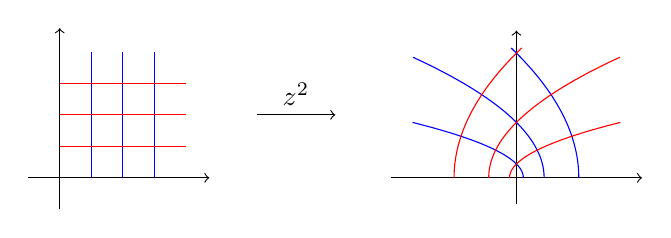
\begin{tikzpicture}
	\begin{scope}
		\draw[->] (-0.4, 0) -- (1.9, 0);
		\draw[->] (0, -0.4) -- (0, 1.9);
		\foreach \c in {0.4, 0.8, 1.2}
			\draw[blue, thin] (\c, 0) -- (\c, 1.6);
		\foreach \c in {0.4, 0.8, 1.2}
			\draw[red, thin] (0, \c) -- (1.6, \c);
	\end{scope}
	\draw[->] (2.5, 0.8) -- (3.5, 0.8) node[pos=0.5, above] {$z^2$};
	\begin{scope}[shift={(5.8,0)}, scale=0.55]
		\draw[->] (-2.9, 0) -- (2.9, 0);
		\draw[->] (0, -0.6) -- (0, 3.4);
		\draw[blue, thin, smooth] plot[domain=0:1.60, variable=\t] ({0.16 - \t*\t}, {0.8*\t});
		\draw[blue, thin, smooth] plot[domain=0:1.74, variable=\t] ({0.64 - \t*\t}, {1.6*\t});
		\draw[blue, thin, smooth] plot[domain=0:1.25, variable=\t] ({1.44 - \t*\t}, {2.4*\t});
		\draw[red, thin, smooth] plot[domain=0:1.60, variable=\t] ({\t*\t - 0.16}, {0.8*\t});
		\draw[red, thin, smooth] plot[domain=0:1.74, variable=\t] ({\t*\t - 0.64}, {1.6*\t});
		\draw[red, thin, smooth] plot[domain=0:1.25, variable=\t] ({\t*\t - 1.44}, {2.4*\t});
	\end{scope}
\end{tikzpicture}
\end{center}
Note also how the first quadrant (the region shown) opens out to fill the whole upper half-plane, in accordance with the doubling of angles at the origin.

Going the other way, fractional powers \emph{open out} sectors. To map the left half-plane $U = \{ \re z < 0\}$ to the wedge $\{-\frac{\pi}{4} < \arg w < \frac{\pi}{4}\}$, we want to halve angles, so we try $z^{1/2}$ -- but we must place the branch cut \emph{outside} $U$, since $z^{1/2}$ is not even continuous, let alone analytic, on its cut. Cutting along the negative imaginary axis and taking $\theta \in (-\frac{\pi}{2}, \frac{3\pi}{2}]$, the map $re^{i\theta} \mapsto \sqrt{r} e^{i\theta/2}$ sends $U$ to the wedge $\frac{\pi}{4} < \arg w < \frac{3\pi}{4}$, and following with a rotation we arrive at
$$
f(z) = -i z^{1/2}.
$$

\textbf{(iii) The exponential.} $w = e^z = e^x e^{iy}$ sends horizontal lines $y = c$ to rays $\arg w = c$, and vertical lines $x = c$ to circles $|w| = e^c$. Consequently it maps a rectangle $x_1 < x < x_2$, $y_1 < y < y_2$ conformally onto a sector of an annulus, and in the degenerate cases:
\begin{itemize}
	\item the horizontal strip $0 < \im z < \pi$ maps to the upper half-plane;
	\item the half-strip $\re z < 0$, $0 < \im z < \pi$ maps to the upper half-disc.
\end{itemize}
\begin{center}
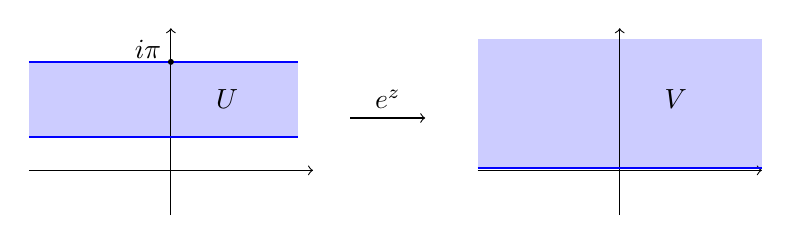
\begin{tikzpicture}[scale=0.95]
	\fill[blue!20] (-1.9, 0.45) rectangle (1.7, 1.45);
	\draw[->] (-1.9, 0) -- (1.9, 0);
	\draw[->] (0, -0.6) -- (0, 1.9);
	\draw[blue, thick] (-1.9, 0.45) -- (1.7, 0.45);
	\draw[blue, thick] (-1.9, 1.45) -- (1.7, 1.45);
	\node[left] at (0, 1.62) {$i\pi$};
	\fill (0, 1.45) circle (0.04);
	\node at (0.75, 0.95) {$U$};
	\draw[->] (2.4, 0.7) -- (3.4, 0.7) node[pos=0.5, above] {$e^z$};
	\begin{scope}[shift={(6,0)}]
		\fill[blue!20] (-1.9, 0.03) rectangle (1.9, 1.75);
		\draw[->] (-1.9, 0) -- (1.9, 0);
		\draw[->] (0, -0.6) -- (0, 1.9);
		\draw[blue, thick] (-1.9, 0.03) -- (1.9, 0.03);
		\node at (0.75, 0.95) {$V$};
	\end{scope}
\end{tikzpicture}
\end{center}
With an appropriate branch, $\log z$ performs the inverse operations, flattening sectors and annuli into strips and rectangles. This pair of maps is the standard tool for `unrolling' angular regions.

\textbf{(iv) M\"obius maps.} As discussed, these shuttle between discs and half-planes. The single most useful example is
$$
f(z) = \frac{z - 1}{z + 1},
$$
which maps the unit disc to the left half-plane. To see this, note the boundary circle passes through $-1 \mapsto \infty$, $i \mapsto i$ and $1 \mapsto 0$, so its image is the circline through $\infty$, $i$, $0$ -- the imaginary axis. Checking an interior point, $f(0) = -1$, so the disc maps to the left half-plane.
\begin{center}
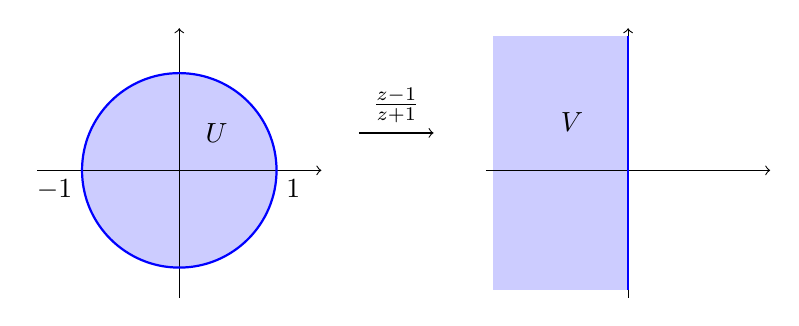
\begin{tikzpicture}[scale=0.95]
	\fill[blue!20] (0,0) circle (1.3);
	\draw[->] (-1.9, 0) -- (1.9, 0);
	\draw[->] (0, -1.7) -- (0, 1.9);
	\draw[blue, thick] (0,0) circle (1.3);
	\node at (0.5, 0.5) {$U$};
	\node[below right] at (1.3, 0) {$1$};
	\node[below left] at (-1.3, 0) {$-1$};
	\draw[->] (2.4, 0.5) -- (3.4, 0.5) node[pos=0.5, above] {$\frac{z-1}{z+1}$};
	\begin{scope}[shift={(6,0)}]
		\fill[blue!20] (-1.8, -1.6) rectangle (0, 1.8);
		\draw[->] (-1.9, 0) -- (1.9, 0);
		\draw[->] (0, -1.7) -- (0, 1.9);
		\draw[blue, thick] (0, -1.6) -- (0, 1.8);
		\node at (-0.75, 0.65) {$V$};
	\end{scope}
\end{tikzpicture}
\end{center}
A useful alternative derivation: $w = \frac{z-1}{z+1}$ rearranges to $z = -\frac{w+1}{w-1}$, and then
$$
|z| < 1 \iff |w + 1| < |w - 1|,
$$
which says exactly that $w$ is closer to $-1$ than to $1$, i.e.\ $\re w < 0$.

The map $z \mapsto 1/z$ is also just a M\"obius map, and is particularly handy for dealing with regions bounded by lines and circles through the origin. For instance, the vertical line $\re z = c$ (with $c > 0$) is a circline through $\infty$ avoiding $0$, so its image under $1/z$ is a circle through the origin; tracking the points $c \mapsto \frac 1c$ and $c \pm i\infty \mapsto 0$, it is the circle of radius $\frac{1}{2c}$ centred at $\frac{1}{2c}$. Consequently $1/z$ maps the half-plane $\re z > c$ to the open disc bounded by that circle -- a useful trick for problems involving two nested or tangent circles.

Let's see the toolkit in action on a composite problem.

\begin{example}[Half-Disc to Disc]
	Let's find a conformal equivalence from the upper half-disc $U = \{|z| < 1, \im z > 0\}$ to the unit disc.

	A tempting first guess is $z \mapsto z^2$, since it maps the upper half-disc onto the disc minus the segment $[0, 1)$ -- but that slit is missing, so this is not onto, and no good. Instead we go via half-planes:
	\begin{enumerate}
		\item $f_1(z) = \frac{z - 1}{z + 1}$ maps $U$ to the second quadrant. (Check: the diameter $(-1, 1)$ maps to the negative real axis, the semicircular arc to the positive imaginary axis, and the interior point $i/2$ maps to $\frac{i/2 - 1}{i/2 + 1} = \frac{-3 + 4i}{5}$, indeed in the second quadrant.)
		\item $f_2(z) = iz^2$: squaring maps the second quadrant to the lower half-plane, and multiplying by $i$ rotates it to the right half-plane.
		\item $f_3(z) = \frac{z-1}{z+1}$ maps the right half-plane to the unit disc: the imaginary axis maps to the unit circle (it is the set of points equidistant from $1$ and $-1$, which maps to $|w| = 1$ by the displayed equivalence above), and $f_3(1) = 0$.
	\end{enumerate}
	The required map is $f_3 \circ f_2 \circ f_1$. One could expand this into a single formula, but there is rarely any reason to.
\end{example}

\begin{example}[Strip to Disc]
	Similarly, let's map the strip $S = \{0 < \im z < 1\}$ conformally onto the unit disc. First scale to the standard strip: $z \mapsto \pi z$ gives $0 < \im z < \pi$. Then exponentiate: $e^z$ maps this strip to the upper half-plane (from the catalogue). Finally, a M\"obius map takes the upper half-plane to the disc: $w \mapsto \frac{w - i}{w + i}$ sends the real axis to the unit circle (each real $w$ is equidistant from $i$ and $-i$) and the interior point $i$ to $0$. Composing,
	$$
	f(z) = \frac{e^{\pi z} - i}{e^{\pi z} + i}.
	$$
	Notice what happened to the boundary: the two edges of the strip, each a copy of $\R$, are wrapped onto complementary arcs of the circle, meeting at the images of the two `ends' of the strip, $f(-\infty) = -1$ and $f(+\infty) = 1$. Keeping track of boundary correspondences like this is exactly what transported the boundary conditions in the Laplace problems below.
\end{example}

\begin{remark}[The Riemann Mapping Theorem]
	One might worry about how far this game can be pushed -- which regions \emph{can} be conformally mapped onto the disc? The answer is remarkably generous: \emph{every} simply connected domain other than $\C$ itself is conformally equivalent to the unit disc (the \emph{Riemann mapping theorem}). The proof is thoroughly non-constructive and belongs to a later course; for us its value is moral support. The map we need always exists -- the examples in this section are about actually finding it.
\end{remark}

\subsection{The Joukowski Map}

One more map deserves special mention, both for its historical importance and because it shows conformal maps doing real engineering work.

\begin{definition}[Joukowski Map]
	The \vocab{Joukowski map} is
	$$
	w = J(z) = \frac{1}{2}\left(z + \frac{1}{z}\right).
	$$
\end{definition}

This is conformal except at $z = \pm 1$, where $J'(z) = \frac{1}{2}(1 - 1/z^2)$ vanishes. Since $J(z) = J(1/z)$, the map is two-to-one on $\C \setminus \{0\}$; it is a conformal equivalence from the \emph{exterior} of the unit circle to the complement of the segment $[-1, 1]$. Indeed, on the unit circle itself $z = e^{i\theta}$ we get $w = \cos\theta$: the circle is flattened onto the segment $[-1, 1]$, traversed twice.

Circles of radius $r > 1$ map to ellipses with semi-axes $\frac{1}{2}(r + \frac 1r)$ and $\frac{1}{2}(r - \frac 1r)$. The magic happens when we apply $J$ to a circle which passes through $z = 1$ but encloses $z = -1$ slightly off-centre: because $J$ fails to be conformal at $z = 1$, the smooth circle acquires a sharp cusp there, and the image is an \emph{aerofoil} -- a wing cross-section with a rounded leading edge and sharp trailing edge.
\begin{center}
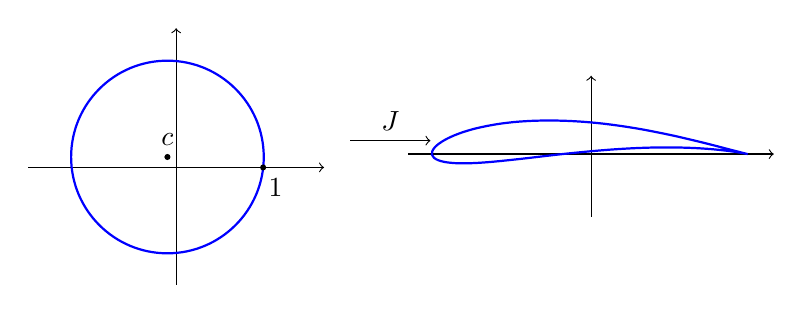
\begin{tikzpicture}[scale=0.85]
	\begin{scope}[shift={(-3.6,0)}, scale=1.3]
		\draw[->] (-1.7, 0) -- (1.7, 0);
		\draw[->] (0, -1.35) -- (0, 1.6);
		\draw[blue, thick] (-0.1, 0.12) circle (1.107);
		\fill (1, 0) circle (0.035);
		\node[below right] at (0.95, -0.02) {$1$};
		\fill (-0.1, 0.12) circle (0.035);
		\node[above, inner sep=4pt] at (-0.1, 0.12) {$c$};
	\end{scope}
	\draw[->] (-1.0, 0.4) -- (0.2, 0.4) node[pos=0.5, above] {$J$};
	\begin{scope}[shift={(2.6,0.2)}, scale=0.78]
		\draw[->] (-3.5, 0) -- (3.5, 0);
		\draw[->] (0, -1.2) -- (0, 1.5);
		\draw[blue, thick, smooth] plot coordinates {(2.979,0.005) (2.905,0.023) (2.781,0.055) (2.612,0.098) (2.403,0.153) (2.159,0.215) (1.886,0.281) (1.589,0.350) (1.272,0.416) (0.941,0.479) (0.599,0.534) (0.252,0.580) (-0.097,0.614) (-0.443,0.635) (-0.782,0.643) (-1.109,0.637) (-1.422,0.618) (-1.717,0.585) (-1.989,0.539) (-2.237,0.484) (-2.456,0.419) (-2.644,0.348) (-2.799,0.273) (-2.919,0.196) (-3.001,0.121) (-3.044,0.049) (-3.047,-0.017) (-3.008,-0.073) (-2.927,-0.119) (-2.804,-0.152) (-2.639,-0.172) (-2.432,-0.178) (-2.185,-0.170) (-1.899,-0.149) (-1.576,-0.117) (-1.221,-0.078) (-0.838,-0.033) (-0.433,0.012) (-0.012,0.053) (0.414,0.088) (0.838,0.113) (1.248,0.126) (1.634,0.126) (1.986,0.115) (2.294,0.095) (2.552,0.069) (2.753,0.043) (2.895,0.020) (2.977,0.005) (3.000,0.000)};
	\end{scope}
\end{tikzpicture}
\end{center}
The point of this construction: we understand ideal fluid flow past a circular cylinder completely (we are about to write it down), and the Joukowski map transports that flow conformally to flow past the aerofoil. This was how early aerodynamicists first computed the lift on a wing.

\subsection{Solving Laplace's Equation with Conformal Maps}

Now we put the machinery to work. The key fact is the one from Section 1: harmonic functions are (locally) real parts of analytic functions, and compositions of analytic functions are analytic. This gives:

\begin{proposition}
	Let $f : U \to V$ be conformal and let $\Phi$ be harmonic on $V$. Then
	$$
	\phi(x, y) = \Phi\big(\re f(x + iy),\ \im f(x + iy)\big)
	$$
	is harmonic on $U$.
\end{proposition}
\begin{proof}
	Since $\Phi$ is harmonic, we can write $\Phi = \re F$ for some analytic $F$ on $V$ (its analytic completion, $F = \Phi + i\Psi$ with $\Psi$ the harmonic conjugate\footnote{On a simply connected domain this always exists; the nice target domains we choose will always be simply connected.}). Then $F \circ f$ is analytic on $U$, being a composition of analytic functions, and $\phi = \re(F \circ f)$ is harmonic.
\end{proof}

In other words: \emph{harmonicity survives conformal changes of variable}. This justifies the following algorithm for solving $\nabla^2 \phi = 0$ on a difficult domain $U$ with given (Dirichlet, say) boundary conditions:
\begin{enumerate}
	\item Find a conformal equivalence $f : U \to V$ with $V$ nice (a half-plane, strip or disc).
	\item Transport the boundary conditions: each boundary point $z \in \partial U$ carries its boundary value over to $f(z) \in \partial V$.
	\item Solve $\nabla^2 \Phi = 0$ on $V$ with the transported boundary conditions -- ideally by inspection.
	\item Then $\phi = \Phi \circ f$ (in the sense of the proposition) solves the original problem.
\end{enumerate}

\begin{example}[Laplace's Equation on a Quadrant]
	Let's find a bounded solution of $\nabla^2 \phi = 0$ on the first quadrant $x, y > 0$, with $\phi(x, 0) = 0$ and $\phi(0, y) = 1$.

	The quadrant is a sector of angle $\frac{\pi}{2}$, so we unroll it with a logarithm: $f(z) = \log z$ (principal branch) maps it to the strip
	$$
	V = \left\{w : 0 < \im w < \frac{\pi}{2}\right\},
	$$
	with the positive real axis (where $\phi = 0$) going to the boundary line $\im w = 0$, and the positive imaginary axis (where $\phi = 1$) to the line $\im w = \frac{\pi}{2}$.

	On the strip, the boundary conditions do not depend on $\re w$, so we look for a solution depending only on $\im w = v$, and $\nabla^2 \Phi = 0$ forces $\Phi$ to be linear in $v$:
	$$
	\Phi(u, v) = \frac{2}{\pi} v.
	$$
	Pulling back,
	$$
	\phi(x, y) = \frac{2}{\pi} \im \log z = \frac{2}{\pi} \arg z = \frac{2}{\pi} \tan^{-1}\left(\frac{y}{x}\right).
	$$
	In hindsight the answer is obvious -- the level sets are rays from the origin, interpolating linearly in angle between the two boundary rays -- but the method required no cleverness, and works just as well when the answer is not guessable.
\end{example}

\begin{example}[Temperature in a Half-Disc]
	Let's solve $\nabla^2 T = 0$ in the upper half-disc $|z| < 1$, $\im z > 0$, with $T = 1$ on the curved boundary and $T = 0$ on the diameter.

	From our catalogue, $f_1(z) = \frac{z-1}{z+1}$ maps the half-disc to the second quadrant, sending the diameter to the negative real axis and the arc to the positive imaginary axis. Then $w = \log\left(\frac{z-1}{z+1}\right)$, taking the branch with $\arg \in [\frac{\pi}{2}, \pi]$ on the closed quadrant, maps the region to the strip $\frac{\pi}{2} < \im w < \pi$, with the arc's image at $\im w = \frac{\pi}{2}$ and the diameter's at $\im w = \pi$. The solution linear in $\im w$ with the right boundary values is $\Phi = 2 - \frac{2}{\pi} \im w$, so
	$$
	T(x, y) = 2 - \frac{2}{\pi}\arg\left(\frac{z - 1}{z + 1}\right).
	$$
	(As always, one should pause and sanity-check: on the arc, $\arg\frac{z-1}{z+1} = \frac{\pi}{2}$ -- the two boundary points $\pm 1$ subtend a right angle from any point of the semicircle -- giving $T = 1$, and on the diameter the argument is $\pi$, giving $T = 0$.)
\end{example}

\begin{example}[Uniform Flow Past a Cylinder]
	As a final showpiece, consider ideal fluid flow, uniform at infinity with speed $U$ parallel to the $x$-axis, past a solid cylinder $|z| \leq a$. We claim the complex potential is
	$$
	w(z) = U\left(z + \frac{a^2}{z}\right).
	$$
	Why: this is analytic in the flow region $|z| > a$; as $z \to \infty$, $w'(z) = U(1 - a^2/z^2) \to U$, giving the right behaviour at infinity; and on the boundary circle $z = ae^{i\theta}$,
	$$
	w = U(ae^{i\theta} + ae^{-i\theta}) = 2Ua\cos\theta,
	$$
	which is real -- so the stream function $\psi = \im w$ vanishes on the cylinder, making it a streamline, as a solid boundary must be. (Notice this is just a scaled Joukowski map!) The stream function is
	$$
	\psi(x, y) = Uy \left(1 - \frac{a^2}{x^2 + y^2}\right),
	$$
	and the streamlines $\psi = \text{const}$ look as follows.
	\begin{center}
	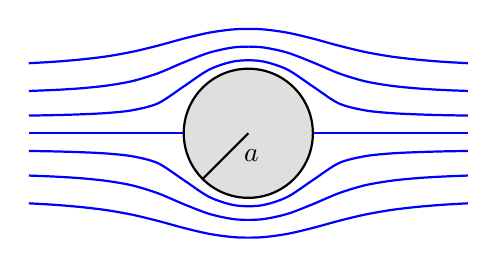
\begin{tikzpicture}[scale=0.82]
		\draw[blue, thick, smooth] plot coordinates {(-3.400,0.274) (-3.000,0.281) (-2.600,0.293) (-2.200,0.313) (-1.800,0.356) (-1.400,0.463) (-1.000,0.725) (-0.600,0.989) (-0.200,1.117) (0.200,1.117) (0.600,0.989) (1.000,0.725) (1.400,0.463) (1.800,0.356) (2.200,0.313) (2.600,0.293) (3.000,0.281) (3.400,0.274)};
		\draw[blue, thick, smooth] plot coordinates {(-3.400,0.655) (-3.000,0.671) (-2.600,0.696) (-2.200,0.737) (-1.800,0.807) (-1.400,0.929) (-1.000,1.098) (-0.600,1.250) (-0.200,1.333) (0.200,1.333) (0.600,1.250) (1.000,1.098) (1.400,0.929) (1.800,0.807) (2.200,0.737) (2.600,0.696) (3.000,0.671) (3.400,0.655)};
		\draw[blue, thick, smooth] plot coordinates {(-3.400,1.085) (-3.000,1.108) (-2.600,1.142) (-2.200,1.190) (-1.800,1.261) (-1.400,1.357) (-1.000,1.466) (-0.600,1.559) (-0.200,1.611) (0.200,1.611) (0.600,1.559) (1.000,1.466) (1.400,1.357) (1.800,1.261) (2.200,1.190) (2.600,1.142) (3.000,1.108) (3.400,1.085)};
		\draw[blue, thick, smooth] plot coordinates {(-3.400,-0.274) (-3.000,-0.281) (-2.600,-0.293) (-2.200,-0.313) (-1.800,-0.356) (-1.400,-0.463) (-1.000,-0.725) (-0.600,-0.989) (-0.200,-1.117) (0.200,-1.117) (0.600,-0.989) (1.000,-0.725) (1.400,-0.463) (1.800,-0.356) (2.200,-0.313) (2.600,-0.293) (3.000,-0.281) (3.400,-0.274)};
		\draw[blue, thick, smooth] plot coordinates {(-3.400,-0.655) (-3.000,-0.671) (-2.600,-0.696) (-2.200,-0.737) (-1.800,-0.807) (-1.400,-0.929) (-1.000,-1.098) (-0.600,-1.250) (-0.200,-1.333) (0.200,-1.333) (0.600,-1.250) (1.000,-1.098) (1.400,-0.929) (1.800,-0.807) (2.200,-0.737) (2.600,-0.696) (3.000,-0.671) (3.400,-0.655)};
		\draw[blue, thick, smooth] plot coordinates {(-3.400,-1.085) (-3.000,-1.108) (-2.600,-1.142) (-2.200,-1.190) (-1.800,-1.261) (-1.400,-1.357) (-1.000,-1.466) (-0.600,-1.559) (-0.200,-1.611) (0.200,-1.611) (0.600,-1.559) (1.000,-1.466) (1.400,-1.357) (1.800,-1.261) (2.200,-1.190) (2.600,-1.142) (3.000,-1.108) (3.400,-1.085)};
		\draw[blue, thick] (-3.4, 0) -- (-1, 0);
		\draw[blue, thick] (1, 0) -- (3.4, 0);
		\draw[thick, fill=gray!25] (0,0) circle (1);
		\draw[thick] (0,0) -- (-0.707, -0.707);
		\node at (0.05, -0.35) {$a$};
	\end{tikzpicture}
	\end{center}
	The velocity on the boundary is $|w'(ae^{i\theta})| = 2U|\sin\theta|$: the flow is stationary at the front and rear \emph{stagnation points} $\theta = 0, \pi$, and fastest at the top and bottom. Composing with a Joukowski-type map now transports this entire flow field to the flow past an aerofoil, streamline by streamline -- conformality guarantees the boundary remains a streamline.
\end{example}

\begin{example}[Flow in a Corner]
	Conformal maps also generate flows directly: if $w(z)$ is a complex potential for a flow in a region $V$, and $g : U \to V$ is conformal, then $w \circ g$ is a complex potential in $U$ (it is analytic, and boundary streamlines pull back to boundary streamlines).

	Uniform flow in the upper half-plane has potential $w(z) = Uz$. The map $g(z) = z^2$ takes the quarter-plane $x, y > 0$ to the upper half-plane. So
	$$
	w(z) = U z^2 = U(x^2 - y^2) + 2iUxy
	$$
	is the potential for flow in a right-angled corner: the stream function is $\psi = 2Uxy$, whose level curves are the hyperbolas $xy = \text{const}$, sliding along the two walls (which form the streamline $\psi = 0$). The velocity $w'(z) = 2Uz$ vanishes at the corner itself -- a stagnation point, as the geometry demands. More generally $w = Uz^{\pi/\phi}$ describes flow in a corner of opening angle $\phi$, and the exponent controls the (in)famous behaviour of the velocity at the vertex: for $\phi > \pi$ (flow around a protruding edge) the velocity is infinite there.
\end{example}

The same technique solves electrostatics problems: the potential between conductors held at fixed voltages is harmonic with Dirichlet boundary conditions, so we conformally map the gap between the conductors to a strip or annulus where the potential is obvious, and pull back. The half-disc example above, reread with `temperature' replaced by `potential' and the boundaries by conductors, is already such an example. Here is one more, with cylindrical rather than flat geometry.

\begin{example}[A Coaxial Cable]
	Two conducting cylinders, radii $r_1 < r_2$, are held at potentials $0$ and $V$; we want the potential $\phi$ in the annulus between them. The map $w = \log z$ (any branch, locally) sends the annulus to the vertical strip $\log r_1 < \re w < \log r_2$, and the boundary circles to the strip's edges. In the strip the solution linear in $\re w$ is immediate, and pulling back,
	$$
	\phi = V \, \frac{\log(r/r_1)}{\log(r_2/r_1)}, \qquad r = |z|.
	$$
	Strictly the annulus is not simply connected and $\log z$ is not single-valued on it -- but its \emph{real} part $\log |z|$ is, and that is all the solution uses. The field lines are the level curves of the conjugate $\im \log z = \theta$: radial lines, orthogonal to the equipotential circles, as they must be.
\end{example}

\section{Contour Integration and Cauchy's Theorem}

We now change gears entirely, and spend the rest of the course on the theory of \emph{integration} of complex functions. If differentiating complex functions felt like a modest generalisation of the real theory, integrating them will not: complex integration has a completely different character, dominated by one theorem (Cauchy's), and it leads to computational techniques that look like magic the first few times you see them.

Throughout this part of the course, our treatment runs parallel to the Complex Analysis course. The definitions below are the same as the ones given there; the difference is that we will move quickly to computation, citing my Complex Analysis notes for the careful proofs.

\subsection{Contours and Integrals}

\begin{definition}[Contour]
	A \vocab{curve} $\gamma$ is a continuous map $\gamma : [a, b] \to \C$. A \vocab{contour} is a piecewise smooth curve; it is \vocab{closed} if $\gamma(a) = \gamma(b)$, and \vocab{simple} if it does not intersect itself (except that a closed contour returns to its start).
\end{definition}

\begin{definition}[Contour Integral]
	The \vocab{contour integral} of $f$ along a contour $\gamma$ is
	$$
	\int_\gamma f(z) \dd z = \int_a^b f(\gamma(t)) \, \gamma'(t) \dd t.
	$$
	For a closed contour we sometimes write $\oint_\gamma f(z) \dd z$, and unless stated otherwise closed contours are traversed \emph{anticlockwise}.
\end{definition}

One can check (by the chain rule) that the integral is independent of the parametrisation chosen, so it really is an integral `along the curve'. Equivalently, the integral is a limit of Riemann sums $\sum f(z_k) \, \delta z_k$ over subdivisions of the contour, which is the picture to keep in mind: we sum up values of $f$ weighted by \emph{complex} displacements along the curve.

The elementary properties are what you would expect: the integral is linear in $f$, additive over concatenation of contours, and changes sign if the contour is traversed backwards. The workhorse inequality is the following, which we will use dozens of times.

\begin{lemma}[Estimation Lemma]
	If $|f(z)| \leq M$ on a contour $\gamma$ of length $L$, then
	$$
	\left| \int_\gamma f(z) \dd z \right| \leq ML.
	$$
\end{lemma}
\begin{proof}
	Bounding the Riemann sums, $|\sum f(z_k) \delta z_k| \leq M \sum |\delta z_k| \leq ML$. (A careful proof is in my Complex Analysis notes.)
\end{proof}

In practice this appears as `length times sup', often in asymptotic form: a semicircle of radius $R$ has length $\pi R$, so if $|f| = O(R^{-2})$ on it then the integral is $O(R^{-1}) \to 0$. Estimates of exactly this shape will kill off the `unwanted' parts of our contours in Section 6.

An important question: does a contour integral depend on the contour, or only on its endpoints? For general functions, it certainly depends on the contour.

\begin{example}[Path Dependence]
	Let's integrate $f(z) = \overline z$ from $0$ to $1 + i$ along two different contours: $\gamma_1$, the straight line $\gamma_1(t) = (1 + i)t$ for $t \in [0,1]$; and $\gamma_2$, going along the real axis to $1$ and then vertically up to $1 + i$.

	Along $\gamma_1$:
	$$
	\int_{\gamma_1} \overline z \dd z = \int_0^1 \overline{(1+i)t} \cdot (1 + i) \dd t = |1 + i|^2 \int_0^1 t \dd t = 1.
	$$
	Along $\gamma_2$: on the horizontal leg $z = t$, $\overline z = t$, contributing $\int_0^1 t \dd t = \frac 12$; on the vertical leg $z = 1 + it$, $\dd z = i \dd t$, contributing $\int_0^1 (1 - it) i \dd t = i + \frac{1}{2}$. Total: $1 + i$.

	So the two routes disagree -- unsurprisingly, since $\overline z$ is not analytic. Repeating the computation with the analytic function $f(z) = z$ gives $\frac{(1+i)^2}{2} = i$ along \emph{both} routes (as the reader should check). Path-independence for analytic functions is not an accident; it is Cauchy's theorem, to which we are heading.
\end{example}

For functions with an antiderivative, the fundamental theorem of calculus works exactly as over $\R$:

\begin{proposition}[Fundamental Theorem of Calculus]
	If $F$ is analytic on a domain containing the contour $\gamma$ from $a$ to $b$, and $F' = f$, then
	$$
	\int_\gamma f(z) \dd z = F(b) - F(a).
	$$
	In particular the integral depends only on the endpoints, and vanishes if $\gamma$ is closed.
\end{proposition}
\begin{proof}
	Parametrise $\gamma$ over $[t_0, t_1]$ and apply the chain rule: $\int_{t_0}^{t_1} f(\gamma(t))\gamma'(t) \dd t = \int_{t_0}^{t_1} \frac{\dd}{\dd t} F(\gamma(t)) \dd t = F(b) - F(a)$.
\end{proof}

\begin{example}[A Fundamental Computation]
	Let $\gamma$ be the circle of radius $r$ about the origin, traversed anticlockwise, and let $n \in \Z$. Parametrising $\gamma(\theta) = re^{i\theta}$,
	$$
	\oint_\gamma z^n \dd z = \int_0^{2\pi} r^n e^{in\theta} \cdot ir e^{i\theta} \dd \theta = i r^{n+1}\int_0^{2\pi} e^{i(n+1)\theta} \dd\theta =
	\begin{cases}
		2\pi i & n = -1, \\
		0 & n \neq -1.
	\end{cases}
	$$
	This tiny computation is secretly the entire subject. Every power of $z$ integrates to zero around a closed loop -- except $\frac 1z$, which detects the loop and contributes $2\pi i$. The residue theorem in Section 6 is little more than this example dressed up.
\end{example}

Note why $n = -1$ is special: $z^n$ has antiderivative $\frac{z^{n+1}}{n+1}$ for $n \neq -1$, and integrals of functions with (single-valued) antiderivatives around closed loops vanish, by the fundamental theorem of calculus. But the antiderivative of $\frac 1z$ is $\log z$, which is multivalued -- going once around the circle, $\log z$ climbs by $2\pi i$, and that is exactly the value of the integral. Branch cuts and contour integrals are two faces of the same phenomenon.

The same computation viewed through open contours is also instructive. Integrating $\frac 1z$ from $-1$ to $1$ along the semicircle $e^{i\theta}$, $\theta$ from $\pi$ down to $0$, through the \emph{upper} half-plane:
$$
\int_\pi^0 \frac{1}{e^{i\theta}} \, ie^{i\theta} \dd \theta = -i\pi,
$$
while through the \emph{lower} half-plane ($\theta$ from $-\pi$ up to $0$) the answer is $+i\pi$. The two routes differ by $2\pi i$ -- the closed-loop value -- and each individually is `$\log 1 - \log(-1)$' for a different branch of $\log$. Everything is consistent, provided one keeps track of which side of the singularity the contour passes.

\subsection{Cauchy's Theorem}

We need one topological notion.

\begin{definition}[Simply Connected]
	A domain $D$ is \vocab{simply connected} if every closed curve in $D$ encloses only points of $D$ -- informally, $D$ has no holes.
\end{definition}

\begin{theorem}[Cauchy's Theorem]
	If $f$ is analytic on a simply connected domain $D$, then for every closed contour $\gamma$ in $D$,
	$$
	\oint_\gamma f(z) \dd z = 0.
	$$
\end{theorem}
\begin{proof}[Proof (Sketch)]
	This is \emph{the} theorem of the course, and it deserves a real proof -- which is given in my Complex Analysis notes. The quick heuristic, assuming $f'$ continuous, comes from Green's theorem: writing $f = u + iv$ and $\dd z = \dd x + i \dd y$,
	$$
	\oint_\gamma f \dd z = \oint_\gamma (u \dd x - v \dd y) + i \oint_\gamma (v \dd x + u \dd y),
	$$
	and applying Green's theorem to each part turns the integrands into $(-v_x - u_y)$ and $(u_x - v_y)$ respectively over the enclosed region -- both of which vanish by the Cauchy--Riemann equations. The honest proof avoids assuming $f'$ is continuous, and is genuinely harder.
\end{proof}

The hypothesis of simple connectedness is doing real work: it guarantees that $f$ is analytic \emph{everywhere inside} $\gamma$, not just on it. Integrating $\frac 1z$ around the unit circle -- which gave $2\pi i$, not $0$ -- does not contradict the theorem, because no simply connected domain contains the circle while avoiding the singularity at $0$.

Cauchy's theorem has two immediate consequences that we use constantly, usually without comment.

\begin{proposition}[Deformation of Contours]
	\begin{enumerate}[label=(\roman*)]
		\item If $\gamma_1$ and $\gamma_2$ are two contours from $a$ to $b$, and $f$ is analytic on a region containing both and the area between them, then $\int_{\gamma_1} f \dd z= \int_{\gamma_2} f \dd z$.
		\item If $\gamma_1$ and $\gamma_2$ are closed contours, one inside the other, and $f$ is analytic on the region between them, then $\oint_{\gamma_1} f \dd z = \oint_{\gamma_2} f \dd z$.
	\end{enumerate}
\end{proposition}
\begin{proof}
	For (i), the concatenation of $\gamma_1$ with $\gamma_2$ reversed is a closed contour to which Cauchy's theorem applies. For (ii), join the two contours by a thin `cross-cut': the resulting single closed contour encloses only the region between $\gamma_1$ and $\gamma_2$, where $f$ is analytic, so the integral around it vanishes; the two passes along the cross-cut cancel in the limit as it narrows, leaving $\oint_{\gamma_1} - \oint_{\gamma_2} = 0$.
\end{proof}

The slogan for (ii): \emph{contours may be freely deformed, so long as they never cross a singularity}. This is the practical form in which Cauchy's theorem enters computations -- we shrink complicated contours onto small circles around the singularities they enclose.

\subsection{Cauchy's Integral Formula}

\begin{theorem}[Cauchy's Integral Formula]
	Let $f$ be analytic on and inside a simple closed contour $\gamma$, and let $z_0$ lie inside $\gamma$. Then
	$$
	f(z_0) = \frac{1}{2\pi i} \oint_\gamma \frac{f(z)}{z - z_0} \dd z.
	$$
\end{theorem}
\begin{proof}
	The integrand is analytic except at $z_0$, so by deformation we may replace $\gamma$ by the circle $z = z_0 + \epsilon e^{i\theta}$ of small radius $\epsilon$. On this circle,
	$$
	\oint \frac{f(z)}{z - z_0} \dd z = \int_0^{2\pi} \frac{f(z_0 + \epsilon e^{i\theta})}{\epsilon e^{i\theta}} \, i\epsilon e^{i\theta} \dd \theta = i \int_0^{2\pi} f(z_0 + \epsilon e^{i\theta}) \dd \theta \to 2\pi i f(z_0)
	$$
	as $\epsilon \to 0$, by continuity of $f$. Since the left hand side is independent of $\epsilon$, it equals $2\pi i f(z_0)$.
\end{proof}

Pause on how strange this is: the values of an analytic function \emph{everywhere inside} a contour are completely determined by its values \emph{on} the contour. Nothing remotely like this is true for real differentiable functions. It reflects the rigidity of analytic functions -- being differentiable in the complex sense ties all the values together.

Differentiating under the integral sign (which can be justified) gives formulas for all derivatives:
$$
f^{(n)}(z_0) = \frac{n!}{2\pi i} \oint_\gamma \frac{f(z)}{(z - z_0)^{n + 1}} \dd z.
$$
In particular \emph{an analytic function is infinitely differentiable} -- the fact we borrowed back in Section 1 to prove harmonicity. The same formulas power the theory of Taylor series, to which we now turn shortly; first, two quick consequences that show off how much information the integral formula packs.

\begin{proposition}[Mean Value Property]
	If $f$ is analytic on a disc about $z_0$, then $f(z_0)$ is the average of $f$ over any circle $|z - z_0| = r$ in the disc:
	$$
	f(z_0) = \frac{1}{2\pi} \int_0^{2\pi} f(z_0 + re^{i\theta}) \dd \theta.
	$$
	Taking real parts, harmonic functions also have the mean value property.
\end{proposition}
\begin{proof}
	Apply Cauchy's integral formula on the circle and parametrise, exactly as in its proof (this time with no limit needed).
\end{proof}

\begin{theorem}[Liouville's Theorem]
	A bounded entire function is constant.
\end{theorem}
\begin{proof}
	Say $|f| \leq M$ everywhere. For any $z_0$, apply the derivative formula on a circle of radius $R$ about $z_0$ and estimate:
	$$
	|f'(z_0)| = \left|\frac{1}{2\pi i} \oint \frac{f(z)}{(z - z_0)^2} \dd z\right| \leq \frac{1}{2\pi} \cdot 2\pi R \cdot \frac{M}{R^2} = \frac MR \to 0
	$$
	as $R \to \infty$. So $f' \equiv 0$, and $f$ is constant.
\end{proof}

Liouville's theorem is the standard route to the fundamental theorem of algebra (if a polynomial $P$ had no root, $1/P$ would be a bounded entire function), and for us it also explains a fact we keep using implicitly: interesting entire functions -- $e^z$, $\sin z$ -- \emph{must} be unbounded somewhere. Both results, along with much more in this vein (Morera's theorem, the identity theorem, the maximum modulus principle), are treated properly in my Complex Analysis notes.

\section{Laurent Series and Singularities}

Analytic functions are exactly the functions given locally by power series -- and near their singularities, they are given by power series allowing negative powers. This section sets up that machinery and uses it to classify singularities, which is precisely what we need to compute residues efficiently.

\subsection{Taylor and Laurent Series}

\begin{theorem}[Taylor Series]
	If $f$ is analytic on the disc $|z - z_0| < R$, then on that disc
	$$
	f(z) = \sum_{n = 0}^\infty a_n (z - z_0)^n, \qquad a_n = \frac{f^{(n)}(z_0)}{n!} = \frac{1}{2\pi i}\oint_\gamma \frac{f(z)}{(z - z_0)^{n+1}} \dd z,
	$$
	where $\gamma$ is any simple closed contour in the disc encircling $z_0$. The series converges (uniformly on compact subsets) in the disc.
\end{theorem}

The proof (expand $\frac{1}{z - w}$ as a geometric series inside Cauchy's integral formula and integrate term by term) is in my Complex Analysis notes. Note the remarkable strength of the statement compared with the real case: mere differentiability guarantees an everywhere-convergent local power series. There is no complex analogue of the smooth-but-not-analytic function $e^{-1/x^2}$.

\begin{example}
	The classics, valid for all $z \in \C$:
	$$
	e^z = \sum_{n=0}^\infty \frac{z^n}{n!}, \qquad
	\sin z = \sum_{n=0}^\infty \frac{(-1)^n z^{2n+1}}{(2n+1)!}, \qquad
	\cos z = \sum_{n=0}^\infty \frac{(-1)^n z^{2n}}{(2n)!},
	$$
	and for $|z| < 1$,
	$$
	\frac{1}{1 - z} = \sum_{n = 0}^\infty z^n, \qquad \log(1 + z) = \sum_{n=1}^\infty \frac{(-1)^{n+1} z^n}{n}
	$$
	(principal branch). The radius of convergence of a Taylor series is always the distance from $z_0$ to the nearest singularity -- which finally explains a real-analysis mystery, namely why $\frac{1}{1 + x^2}$, a perfectly smooth function on all of $\R$, has Taylor series with radius of convergence only $1$: the function has (complex!) singularities at $\pm i$, at distance $1$ from the origin.
\end{example}

What if $f$ has a singularity at $z_0$ itself, or we are working in an annulus around a hole? We then allow negative powers.

\begin{theorem}[Laurent Series]
	If $f$ is analytic in an annulus $R_1 < |z - z_0| < R_2$, then on that annulus
	$$
	f(z) = \sum_{n = -\infty}^{\infty} a_n (z - z_0)^n, \qquad a_n = \frac{1}{2\pi i} \oint_\gamma \frac{f(z)}{(z - z_0)^{n + 1}} \dd z,
	$$
	where $\gamma$ is any simple closed contour in the annulus encircling $z_0$. The expansion is unique, and converges uniformly on compact subsets of the annulus.
\end{theorem}

Uniqueness is worth emphasising for practical reasons: \emph{any} valid method of producing such an expansion -- long division, substituting into known series, partial fractions -- must give \emph{the} Laurent series. We never compute the coefficient integrals directly.

\begin{example}[Computing Laurent Series]
	\begin{enumerate}[label=(\roman*)]
		\item Around $z_0 = 0$,
		$$
		\frac{e^z}{z^3} = \frac{1}{z^3}\left(1 + z + \frac{z^2}{2} + \cdots\right) = \frac{1}{z^3} + \frac{1}{z^2} + \frac{1}{2z} + \frac{1}{6} + \frac{z}{24} + \cdots.
		$$
		\item $e^{1/z}$ has Laurent series $\sum_{n=0}^\infty \frac{z^{-n}}{n!}$ around $0$, with \emph{infinitely many} negative powers.
		\item The function $\frac{1}{z(z-1)}$ has \emph{different} Laurent expansions in the annuli $0 < |z| < 1$ and $|z| > 1$:
		$$
		\frac{1}{z(z - 1)} = -\frac{1}{z} \cdot \frac{1}{1 - z} = -\frac 1z - 1 - z - z^2 - \cdots \qquad (0 < |z| < 1),
		$$
		while for $|z| > 1$ we expand in powers of $\frac 1z$ instead:
		$$
		\frac{1}{z(z-1)} = \frac{1}{z^2} \cdot \frac{1}{1 - 1/z} = \frac{1}{z^2} + \frac{1}{z^3} + \frac{1}{z^4} + \cdots.
		$$
		Same function, same centre, different annuli, different series -- uniqueness is per-annulus.
		\item Expansions about points other than the singularity work the same way. For $\frac{1}{z(z-2)}$ about $z_0 = 1$: writing $\zeta = z - 1$,
		$$
		\frac{1}{z(z - 2)} = \frac{1}{(\zeta + 1)(\zeta - 1)} = \frac{1}{\zeta^2 - 1} = -\left(1 + \zeta^2 + \zeta^4 + \cdots\right) \qquad (|\zeta| < 1)
		$$
		-- a Taylor series, no negative powers, since the function is analytic at $z = 1$; the nearest singularities (at $0$ and $2$) set the radius of convergence to $1$. In the outer region $|\zeta| > 1$ we would instead expand in $\frac{1}{\zeta}$ and find only negative powers.
	\end{enumerate}
\end{example}

\subsection{Zeros and the Classification of Singularities}

\begin{definition}[Order of a Zero]
	A \vocab{zero} of an analytic function $f$ is a point with $f(z_0) = 0$. Its \vocab{order} is the index of the first non-vanishing Taylor coefficient at $z_0$; a zero of order 1 is called \vocab{simple}.
\end{definition}

So $z^3 + iz = z(z^2 + i)$ has a simple zero at the origin (and at the two square roots of $-i$), and $\sinh^3 z$ has a zero of order 3 at $z = n\pi i$ for each $n \in \Z$. Zeros of order $k$ look locally like $c(z - z_0)^k$.

\begin{definition}[Isolated Singularity]
	If $f$ is analytic on a punctured neighbourhood $0 < |z - z_0| < r$ of $z_0$ but not at $z_0$ itself, then $z_0$ is an \vocab{isolated singularity} of $f$.
\end{definition}

Branch points are the standard example of \emph{non}-isolated singularities in this course -- there is no punctured neighbourhood of a branch point on which the function is even single-valued, so no Laurent expansion exists there. At an isolated singularity, however, we have a Laurent series, and we classify the singularity by how badly the series fails to be a Taylor series. Suppose $f(z) = \sum_{n=-\infty}^{\infty} a_n (z - z_0)^n$ on $0 < |z - z_0| < r$.

\begin{enumerate}[label=(\roman*)]
	\item If $a_n = 0$ for all $n < 0$, then $z_0$ is a \vocab{removable singularity}: defining $f(z_0) = a_0$ extends $f$ analytically across $z_0$. Example: $\frac{\sin z}{z}$ at $0$.
	\item If $a_n = 0$ for $n < -N$ but $a_{-N} \neq 0$ (some $N \geq 1$), then $z_0$ is a \vocab{pole of order $N$}. Poles of order $1, 2, 3$ are called \emph{simple, double, triple}. Example: $\frac{e^z}{z^3}$ has a triple pole at $0$, as we computed. Near a pole, $|f(z)| \to \infty$.
	\item Otherwise -- infinitely many negative coefficients -- $z_0$ is an \vocab{essential singularity}. Example: $e^{1/z}$ at $0$.
\end{enumerate}

Poles are the well-behaved singularities, and essentially all singularities met in this course are poles. Note $f$ has a pole of order $N$ at $z_0$ exactly when $\frac{1}{f}$ has a zero of order $N$ there (poles of $f$ are zeros of $1/f$ and vice versa), which is usually the fastest way to find the order of a pole: for instance $\frac{1}{\sinh^3 z}$ has a triple pole at each $z = n\pi i$.

Essential singularities are genuinely wild: in any neighbourhood of an essential singularity, $f$ takes values arbitrarily close to \emph{every} complex number (Casorati--Weierstrass; Picard proved the stronger statement that it takes every value with at most one exception, infinitely often). We will treat this as a good reason to stay away from them.

Let's practice the classification -- this is the sort of thing one must be able to do at sight.

\begin{example}[Classifying Singularities]
	\begin{enumerate}[label=(\roman*)]
		\item $\dfrac{z}{\sin z}$: at $z = 0$, both numerator and denominator have simple zeros, so the singularity is \emph{removable} (with value $1$). At $z = n\pi$ for $n \neq 0$, the denominator has a simple zero and the numerator doesn't vanish: \emph{simple poles}.
		\item $\tan z = \dfrac{\sin z}{\cos z}$: simple poles at the zeros $\left(n + \frac 12\right)\pi$ of $\cos$, each with residue $\frac{\sin z}{-\sin z} = -1$ by the $\frac{g}{h'}$ rule (coming shortly).
		\item $\dfrac{\cos z - 1}{z^4}$: the numerator has a \emph{double} zero at $0$ (its series starts at $-\frac{z^2}{2}$), so this is a double pole, with Laurent series $-\frac{1}{2z^2} + \frac{1}{24} - \cdots$. Note the residue is $0$ -- poles can have zero residue.
		\item $\sin \frac 1z$: essential singularity at $0$ (the Laurent series $\frac 1z - \frac{1}{3! z^3} + \cdots$ has infinitely many negative terms).
		\item $\dfrac{1}{\sin(1/ z)}$: this has simple poles at $z = \frac{1}{n\pi}$, which \emph{accumulate} at $0$. So $z = 0$ is a singularity but not an isolated one -- there is no punctured disc around $0$ free of other singularities -- and it is therefore none of the three types. No Laurent series about $0$ exists.
	\end{enumerate}
\end{example}

\begin{remark}[Behaviour at Infinity]
	As always, we classify the point at infinity by looking at $f(1/z)$ at $0$. A polynomial of degree $n$ has a pole of order $n$ at $\infty$; a rational function is analytic at $\infty$ iff its denominator degree is at least its numerator degree; and $e^z$ has an \emph{essential} singularity at $\infty$ (as $e^{1/z}$ does at $0$) -- which is one way to understand why $e^z$ attains every non-zero value in every half-plane $\re z > R$.
\end{remark}

\subsection{Residues}

For the applications, one Laurent coefficient towers above the rest in importance.

\begin{definition}[Residue]
	The \vocab{residue} of $f$ at an isolated singularity $z_0$ is the coefficient $a_{-1}$ of its Laurent expansion about $z_0$, written $\Res_{z = z_0} f(z)$.
\end{definition}

Why single out $a_{-1}$? Integrate the Laurent series term by term around a small circle about $z_0$: by our fundamental computation, every term dies except the $\frac{1}{z - z_0}$ term, and
$$
\oint f(z) \dd z = 2\pi i \, a_{-1}.
$$
So the residue is exactly what survives integration. This observation \emph{is} the residue theorem, up to bookkeeping; but before stating it, let's build the toolkit for computing residues without ever writing down a full Laurent expansion.

\begin{proposition}[Computing Residues]
	Let $z_0$ be a pole of $f$.
	\begin{enumerate}[label=(\roman*)]
		\item If the Laurent series is available or easy, read off $a_{-1}$.
		\item If $z_0$ is a simple pole,
		$$
		\Res_{z = z_0} f(z) = \lim_{z \to z_0} (z - z_0) f(z).
		$$
		\item If $f = \frac{g}{h}$ with $g(z_0) \neq 0$ and $h$ having a simple zero at $z_0$, then
		$$
		\Res_{z = z_0} f(z) = \frac{g(z_0)}{h'(z_0)}.
		$$
		\item If $z_0$ is a pole of order $N$,
		$$
		\Res_{z = z_0} f(z) = \lim_{z \to z_0} \frac{1}{(N-1)!} \frac{\dd^{N - 1}}{\dd z^{N - 1}} \Big( (z - z_0)^N f(z) \Big).
		$$
	\end{enumerate}
\end{proposition}
\begin{proof}
	For (ii) and (iv), write out the Laurent series: $(z - z_0)^N f(z) = a_{-N} + a_{-N + 1}(z - z_0) + \cdots$ is analytic at $z_0$, and differentiating $N - 1$ times and evaluating at $z_0$ isolates $(N-1)! \, a_{-1}$. For (iii), note
	$$
	\lim_{z \to z_0} (z - z_0)\frac{g(z)}{h(z)} = g(z_0) \lim_{z \to z_0} \frac{z - z_0}{h(z) - h(z_0)} = \frac{g(z_0)}{h'(z_0)}. \qedhere
	$$
\end{proof}

Method (iii) is used more than all the others combined. A quick gallery:

\begin{example}[Computing Residues]
	\begin{enumerate}[label=(\roman*)]
		\item $\dfrac{e^z}{z^3}$ at $z = 0$: from the Laurent series above, the residue is $\frac{1}{2}$.
		\item $\dfrac{1}{1 + z^4}$ at $z_0 = e^{i\pi/4}$: by (iii), the residue is $\frac{1}{4z_0^3} = \frac{z_0}{4z_0^4} = -\frac{1}{4}e^{i\pi/4}$. (Multiplying top and bottom by $z_0$ to use $z_0^4 = -1$ is a trick worth remembering.)
		\item $\dfrac{e^{iz}}{\sinh z}$ at $z = \pi i$: $\sinh$ has a simple zero there, so by (iii) the residue is $\frac{e^{i \cdot \pi i}}{\cosh \pi i} = \frac{e^{-\pi}}{\cos \pi} = -e^{-\pi}$.
		\item $\dfrac{1}{(z^2 + a^2)^2}$ at $z = ia$ (a double pole, $a > 0$): by (iv),
		$$
		\Res_{z = ia} = \lim_{z \to ia} \frac{\dd}{\dd z} \frac{1}{(z + ia)^2} = \frac{-2}{(2ia)^3} = -\frac{i}{4a^3}.
		$$
		\item Essential singularities have residues too -- the definition only needs the Laurent coefficient -- but the pole formulas above do not apply, and one must go back to the series. For instance $e^{1/z}$ has residue $1$ at the origin (the $n = 1$ term of $\sum \frac{z^{-n}}{n!}$), and $z e^{1/z}$, whose expansion $z + 1 + \frac{1}{2z} + \cdots$ has residue $\frac 12$.
	\end{enumerate}
\end{example}

\section{The Calculus of Residues}

This section contains the computational heart of the course. The residue theorem turns the evaluation of contour integrals into the algebra of computing residues -- and with the right contours, an enormous variety of \emph{real} integrals fall to it. The section is essentially a sequence of worked examples, each illustrating a standard contour or trick; between them they cover everything that appears on example sheets and exams.

\subsection{The Residue Theorem}

\begin{theorem}[Residue Theorem]
	Let $f$ be analytic on and inside a simple closed contour $\gamma$ (traversed anticlockwise), except at finitely many isolated singularities $z_1, \dots, z_n$ inside $\gamma$. Then
	$$
	\oint_\gamma f(z) \dd z = 2\pi i \sum_{k = 1}^n \Res_{z = z_k} f(z).
	$$
\end{theorem}
\begin{proof}
	Deform $\gamma$, without crossing any singularity, into small circles $\gamma_k$ around each $z_k$ joined by cross-cuts (the cross-cut contributions cancel in pairs as they narrow, exactly as in the proof of contour deformation). This gives
	$$
	\oint_\gamma f(z) \dd z = \sum_{k=1}^n \oint_{\gamma_k} f(z) \dd z.
	$$
	On each small circle, integrate the Laurent expansion of $f$ about $z_k$ term by term: every power of $(z - z_k)$ integrates to zero except the $(-1)$-th, which gives $2\pi i \, a_{-1} = 2\pi i \Res_{z = z_k} f$.
\end{proof}

A fully rigorous version of this argument (with winding numbers, and without the appeal to pictures) is in my Complex Analysis notes. For this course, the picture \emph{is} the point: the integral around $\gamma$ only sees the singularities inside, each contributing $2\pi i$ times its residue.

Everything else in this section is technique for \emph{choosing} $\gamma$.

\subsection{Integrals Along the Real Axis}

The prototype problem: evaluate $\int_{-\infty}^\infty f(x) \dd x$ for a rational function $f$ decaying at infinity. The strategy is to `close the contour': integrate $f(z)$ around the contour consisting of the real segment $[-R, R]$ together with the semicircle $\gamma_R$ of radius $R$ in the upper half-plane, apply the residue theorem, and let $R \to \infty$, arguing that the semicircle's contribution dies.

\begin{center}
\begin{tikzpicture}[scale=0.95]
	\draw[->] (-3, 0) -- (3, 0);
	\draw[->] (0, -0.7) -- (0, 2.9);
	\draw[blue, thick, ->-=0.25, ->-=0.75] (-2.1, 0) -- (2.1, 0) arc (0:180:2.1);
	\node[below] at (-2.1, 0) {$-R$};
	\node[below] at (2.1, 0) {$R$};
	\node[blue] at (1.05, -0.32) {$\gamma_0$};
	\node[blue] at (1.9, 1.75) {$\gamma_R$};
	\node at (0, 1) {$\times$};
	\node[right] at (0.1, 1) {$i$};
\end{tikzpicture}
\end{center}

\begin{example}[The Prototype]
	Let's evaluate
	$$
	I = \int_0^\infty \frac{\dd x}{1 + x^2}.
	$$
	Of course we know the answer is $\arctan \infty = \frac{\pi}{2}$; the point is to establish the method on familiar ground. Consider
	$$
	\oint_\gamma \frac{\dd z}{1 + z^2}
	$$
	around the contour above. The integrand factors as $\frac{1}{(z-i)(z+i)}$, so the only enclosed singularity is the simple pole at $z = i$, with residue $\frac{1}{2i}$. The residue theorem gives, for all $R > 1$,
	$$
	\int_{\gamma_0} \frac{\dd z}{1 + z^2} + \int_{\gamma_R} \frac{\dd z}{1 + z^2} = 2\pi i \cdot \frac{1}{2i} = \pi.
	$$
	As $R \to \infty$, the first integral tends to $\int_{-\infty}^\infty \frac{\dd x}{1 + x^2} = 2I$ by evenness. For the second, on $\gamma_R$ we have $|1 + z^2| \geq R^2 - 1$, so by the estimation lemma
	$$
	\left|\int_{\gamma_R} \frac{\dd z}{1 + z^2}\right| \leq \frac{\pi R}{R^2 - 1} \to 0.
	$$
	Hence $2I = \pi$, so $I = \frac{\pi}{2}$ as expected.
\end{example}

Some remarks before the next examples, all of them important for practice:
\begin{enumerate}[label=(\roman*)]
	\item The informal version of the tail estimate, universally used: on $\gamma_R$, the integrand is $O(R^{-2})$ and the contour has length $\pi R$, so the integral is $O(R^{-1}) \to 0$. Any rational function with denominator degree exceeding numerator degree by at least $2$ dies this way.
	\item We could equally have closed in the \emph{lower} half-plane. The enclosed pole is then $-i$ with residue $-\frac{1}{2i}$, but the contour is traversed clockwise, contributing a compensating sign: same answer. Close wherever the estimate works; when both work, pick whichever contains nicer poles.
	\item The method's value is its generality -- replace $1 + x^2$ by $1 + x^8$ and the trigonometric substitution collapses, but the contour argument goes through verbatim.
\end{enumerate}

\begin{example}[A Double Pole]
	For $a > 0$,
	$$
	\int_0^\infty \frac{\dd x}{(x^2 + a^2)^2}.
	$$
	Same contour. The only enclosed singularity is the \emph{double} pole at $z = ia$, whose residue we computed in Section 5: $-\frac{i}{4a^3}$. The semicircle integrand is $O(R^{-4})$, so its integral is $O(R^{-3}) \to 0$, and
	$$
	2I = 2\pi i \left(-\frac{i}{4 a^3}\right) = \frac{\pi}{2a^3}, \qquad I = \frac{\pi}{4a^3}.
	$$
\end{example}

\begin{example}[Choosing a Cleverer Contour]
	Consider
	$$
	I = \int_0^\infty \frac{\dd x}{1 + x^4}.
	$$
	The semicircular contour works: the enclosed poles are $e^{i\pi/4}$ and $e^{3i\pi/4}$, with residues $-\frac{1}{4}e^{i\pi/4}$ and $-\frac{1}{4}e^{3i\pi/4}$ (using the $\frac{g}{h'}$ formula and the $z_0^4 = -1$ trick), giving after a little algebra $I = \frac{\pi}{2\sqrt 2}$.

	But since the integrand has the symmetry $f(iz) = f(z)$, there is a slicker choice: the quarter-circle contour $0 \to R \to iR \to 0$ (out along the real axis, around the arc, back down the imaginary axis). The return leg contributes, substituting $z = iy$,
	$$
	\int_R^0 \frac{i \dd y}{1 + y^4} \to -iI,
	$$
	the arc dies as usual, and only the single pole $e^{i\pi/4}$ is enclosed. So
	$$
	(1 - i) I = 2\pi i \left(-\tfrac 14 e^{i\pi/4}\right), \qquad I = \frac{-\frac{\pi i}{2} e^{i \pi /4}}{1 - i} = \frac{\pi}{2\sqrt{2}},
	$$
	with less residue arithmetic. Matching the contour to the symmetry of the integrand is a recurring theme.
\end{example}

\begin{example}[A Wedge Contour]
	The quarter-circle idea generalises to any integrand with a rotational symmetry. Consider
	$$
	I = \int_0^\infty \frac{\dd x}{1 + x^3}.
	$$
	(Note we \emph{cannot} close a semicircle here: the integrand is not even, so $\int_{-\infty}^\infty$ is not $2I$ -- indeed the integrand has a pole at $x = -1$ on the negative real axis.) The symmetry is $z \mapsto e^{2\pi i/3} z$, which permutes the poles and fixes the integrand. So take the wedge contour: out along the real axis to $R$, around the arc of angle $\frac{2\pi}{3}$, and back along the ray $\arg z = \frac{2\pi}{3}$. On the returning ray, $z = e^{2\pi i /3} t$ gives $1 + z^3 = 1 + t^3$ and $\dd z = e^{2\pi i/3} \dd t$, so that leg contributes $-e^{2\pi i /3} I$; the arc dies as $O(R^{-2})$.

	The wedge encloses exactly one pole, $z_0 = e^{i\pi/3}$, with residue $\frac{1}{3z_0^2} = \frac{z_0}{3 z_0^3} = -\frac{z_0}{3}$. Hence
	$$
	(1 - e^{2\pi i /3}) I = -\frac{2\pi i}{3} e^{i\pi/3},
	$$
	and factoring $1 - e^{2\pi i/3} = -e^{i\pi/3}(e^{i\pi/3} - e^{-i\pi/3}) = -2i e^{i\pi/3}\sin\frac\pi 3$,
	$$
	I = \frac{\pi/3}{\sin(\pi/3)} = \frac{2\pi}{3\sqrt 3}.
	$$
	The same wedge of angle $\frac{2\pi}{n}$ handles $\int_0^\infty \frac{\dd x}{1 + x^n}$ for any $n \geq 2$, giving $\frac{\pi/n}{\sin(\pi/n)}$.
\end{example}

\begin{example}[The Fresnel Integrals]
	A wedge can rotate an integral onto an axis where it becomes elementary, even with \emph{no poles at all}. The Fresnel integrals
	$$
	\int_0^\infty \cos(x^2) \dd x \quad \text{and} \quad \int_0^\infty \sin(x^2) \dd x
	$$
	(which converge, delicately, by the increasingly rapid oscillation) are the real and imaginary parts of $\int_0^\infty e^{ix^2} \dd x$. Integrate the \emph{entire} function $e^{iz^2}$ around the wedge of angle $\frac{\pi}{4}$: out to $R$, around the arc, and back along the ray $z = e^{i\pi/4} t$. Cauchy's theorem says the total is zero.

	The point of the angle $\frac \pi 4$: on the returning ray, $z^2 = it^2$, so
	$$
	e^{iz^2} = e^{i \cdot it^2} = e^{-t^2},
	$$
	and the wild oscillatory integrand becomes the Gaussian. The ray leg contributes $-e^{i\pi/4}\int_0^R e^{-t^2} \dd t$. On the arc, $|e^{iz^2}| = e^{-R^2 \sin 2\theta}$, and the Jordan-style bound $\sin 2\theta \geq \frac{4\theta}{\pi}$ on $[0, \frac \pi 4]$ gives
	$$
	\left|\int_{\text{arc}}\right| \leq R \int_0^{\pi/4} e^{-4R^2 \theta/\pi} \dd \theta \leq \frac{\pi}{4R} \to 0.
	$$
	Hence, letting $R \to \infty$ and using $\int_0^\infty e^{-t^2} \dd t = \frac{\sqrt \pi}{2}$,
	$$
	\int_0^\infty e^{ix^2} \dd x = e^{i\pi/4} \cdot \frac{\sqrt\pi}{2},
	$$
	and separating real and imaginary parts,
	$$
	\int_0^\infty \cos(x^2) \dd x = \int_0^\infty \sin(x^2) \dd x = \frac 12 \sqrt{\frac{\pi}{2}}.
	$$
	No residues were harmed in this example -- the entire content of the calculation was the freedom to rotate the contour.
\end{example}

\subsection{Trigonometric Integrals}

For integrals of a rational function of $\sin\theta$ and $\cos\theta$ over a full period, no limiting process is needed at all: the unit circle \emph{is} the contour.

Substitute $z = e^{i\theta}$, so that as $\theta$ runs from $0$ to $2\pi$, $z$ traverses the unit circle $\gamma$ anticlockwise, and
$$
\cos \theta = \frac{1}{2}\left(z + \frac 1z\right), \qquad \sin\theta = \frac{1}{2i}\left(z - \frac 1z\right), \qquad \dd \theta = \frac{\dd z}{iz}.
$$

\begin{example}
	For $a > 1$, let's compute
	$$
	I = \int_0^{2\pi} \frac{\dd \theta}{a + \cos\theta}.
	$$
	Substituting,
	$$
	I = \oint_\gamma \frac{1}{a + \frac 12 (z + z^{-1})} \frac{\dd z}{iz} = \frac{2}{i}\oint_\gamma \frac{\dd z}{z^2 + 2az + 1}.
	$$
	The denominator has roots $z_\pm = -a \pm \sqrt{a^2 - 1}$, real, with $z_+ z_- = 1$; since $a > 1$ we have $|z_-| > 1 > |z_+|$, so only $z_+$ is enclosed. Its residue is $\frac{1}{z_+ - z_-} = \frac{1}{2\sqrt{a^2 - 1}}$, and
	$$
	I = \frac{2}{i} \cdot 2\pi i \cdot \frac{1}{2\sqrt{a^2 - 1}} = \frac{2\pi}{\sqrt{a^2 - 1}}.
	$$
\end{example}

\begin{example}[The Poisson Kernel Integral]
	For $|a| < 1$, let's compute
	$$
	I = \int_0^{2\pi} \frac{\dd \theta}{1 - 2a\cos\theta + a^2},
	$$
	which the reader may recognise as the normalisation of the Poisson kernel from IB Methods. The denominator factors beautifully after the substitution: since $1 - 2a\cos\theta + a^2 = (1 - ae^{i\theta})(1 - ae^{-i\theta})$,
	$$
	I = \oint_\gamma \frac{1}{(1 - az)(1 - a/z)} \frac{\dd z}{iz} = \frac 1i \oint_\gamma \frac{\dd z}{(1 - az)(z - a)}.
	$$
	The integrand has simple poles at $z = a$ (inside the unit circle) and $z = \frac 1a$ (outside) -- note how the two poles are inversions of each other, mirroring the symmetry of the original expression. Only $z = a$ contributes:
	$$
	I = \frac 1i \cdot 2\pi i \cdot \frac{1}{1 - a^2} = \frac{2\pi}{1 - a^2}.
	$$
\end{example}

\subsection{Jordan's Lemma}

Integrals like $\int \frac{\cos x}{1 + x^2} \dd x$ bring a new difficulty. To use contour methods we must extend the integrand off the real axis, and the natural-looking extension $\frac{\cos z}{1 + z^2}$ is a trap: $\cos z = \frac{e^{iz} + e^{-iz}}{2}$ grows exponentially as $\im z \to \pm\infty$ (in \emph{both} half-planes!), so no closing semicircle can die. The correct move is to integrate $\frac{e^{iz}}{1 + z^2}$, which is bounded in the upper half-plane since $|e^{iz}| = e^{-\im z}$, and take real parts at the end.

For decay of the semicircle we then need a slightly finer estimate than `length times sup', because $|e^{iz}|$ is only small on \emph{most} of the semicircle -- near the real axis it is of size 1. The right tool:

\begin{lemma}[Jordan's Lemma]
	Let $f$ be analytic in the upper half-plane apart from finitely many singularities, with $f(z) \to 0$ as $|z| \to \infty$. Then for any constant $\lambda > 0$,
	$$
	\int_{\gamma_R} f(z) e^{i\lambda z} \dd z \to 0 \quad \text{as } R \to \infty,
	$$
	where $\gamma_R$ is the semicircle of radius $R$ in the upper half-plane. For $\lambda < 0$ the same holds with the semicircle in the lower half-plane.
\end{lemma}
\begin{proof}
	Parametrise $z = Re^{i\theta}$. The whole point is the bound $|e^{i\lambda z}| = e^{-\lambda R \sin\theta}$, together with the elementary inequality $\sin\theta \geq \frac{2\theta}{\pi}$ on $[0, \frac{\pi}{2}]$ (the sine curve lies above its chord). Splitting the semicircle symmetrically and using this:
	\begin{align*}
		\left|\int_{\gamma_R} f(z) e^{i\lambda z} \dd z\right|
		&\leq R \sup_{z \in \gamma_R}|f(z)| \int_0^\pi e^{-\lambda R \sin\theta} \dd\theta
		\leq 2R \sup_{z \in \gamma_R}|f(z)| \int_0^{\pi/2} e^{-2\lambda R\theta/\pi} \dd \theta \\
		&= \frac{\pi}{\lambda}\left(1 - e^{-\lambda R}\right) \sup_{z \in \gamma_R} |f(z)| \to 0,
	\end{align*}
	since $\sup_{\gamma_R} |f| \to 0$ by hypothesis.
\end{proof}

The lesson to remember alongside the lemma: \emph{the factor $e^{i\lambda z}$ decides which half-plane to close in} -- upper for $\lambda > 0$, lower for $\lambda < 0$. If $f$ decays like $R^{-2}$ we don't need the lemma (crude estimation suffices), but when $f \sim R^{-1}$ -- as for Fourier transforms of rational functions with degree gap 1 -- Jordan's lemma is essential.

\begin{example}
	For $\alpha > 0$, let's find
	$$
	I = \int_0^\infty \frac{\cos \alpha x}{1 + x^2} \dd x.
	$$
	Close $\frac{e^{i\alpha z}}{1 + z^2}$ in the upper half-plane (as $\alpha > 0$). The enclosed pole is $z = i$ with residue $\frac{e^{i\alpha \cdot i}}{2i} = \frac{e^{-\alpha}}{2i}$, so
	$$
	\int_{-\infty}^\infty \frac{e^{i\alpha x}}{1 + x^2} \dd x = 2\pi i \cdot \frac{e^{-\alpha}}{2i} = \pi e^{-\alpha}.
	$$
	Taking real parts and halving (the integrand $\frac{\cos \alpha x}{1+x^2}$ is even; its companion $\frac{\sin \alpha x}{1 + x^2}$ is odd, so the answer was real all along),
	$$
	I = \frac{\pi}{2} e^{-\alpha}.
	$$
	It is worth noticing the answer is \emph{not analytic in $\alpha$} at $0$ -- it is $\frac{\pi}{2}e^{-|\alpha|}$ for real $\alpha$ -- a hint that something interesting (closing in opposite half-planes) happens as $\alpha$ changes sign.
\end{example}

\begin{example}[Where Jordan is Genuinely Needed]
	For $a > 0$, let's compute
	$$
	I = \int_0^\infty \frac{x \sin x}{x^2 + a^2} \dd x.
	$$
	Close $f(z) e^{iz}$ with $f(z) = \frac{z}{z^2 + a^2}$ in the upper half-plane. This time $f \sim \frac 1R$ on the arc, so the crude bound gives $\pi R \cdot O(R^{-1}) = O(1)$ -- useless -- and Jordan's lemma is doing real work. The enclosed pole is $z = ia$:
	$$
	\int_{-\infty}^\infty \frac{x e^{ix}}{x^2 + a^2} \dd x = 2\pi i \Res_{z = ia} \frac{z e^{iz}}{z^2 + a^2} = 2\pi i \cdot \frac{ia \, e^{-a}}{2ia} = \pi i e^{-a}.
	$$
	Taking imaginary parts and halving (the integrand is even),
	$$
	I = \frac{\pi}{2} e^{-a}.
	$$
	(The real part of the identity reads $\pv\int \frac{x\cos x}{x^2 + a^2} \dd x = 0$, correct by oddness.)
\end{example}

\subsection{Indented Contours and Principal Values}

Next complication: a pole \emph{on} the contour. The classic example is
$$
I = \int_{-\infty}^\infty \frac{\sin x}{x} \dd x.
$$
The real integrand is perfectly finite at $x = 0$ (removable singularity), but the function we want to close with, $\frac{e^{iz}}{z}$, has a genuine pole at the origin, sitting exactly on our contour. The fix is to \emph{indent}: walk along the real axis from $-R$ to $-\epsilon$, hop over the pole via a small semicircle $C_\epsilon$ in the upper half-plane, continue from $\epsilon$ to $R$, and close with the big semicircle $C_R$.

\begin{center}
\begin{tikzpicture}[scale=0.95]
	\draw[->] (-3, 0) -- (3, 0);
	\draw[->] (0, -0.7) -- (0, 2.9);
	\draw[blue, thick, ->-=0.1, ->-=0.42, ->-=0.8] (-2.3, 0) -- (-0.45, 0) arc (180:0:0.45) -- (2.3, 0) arc (0:180:2.3);
	\node[below] at (-2.3, 0) {$-R$};
	\node[below] at (2.3, 0) {$R$};
	\node[below] at (-0.55, 0) {$-\epsilon$};
	\node[below] at (0.62, 0) {$\epsilon$};
	\node[blue] at (-0.62, 0.62) {$C_\epsilon$};
	\node[blue] at (2.05, 1.9) {$C_R$};
	\node at (0, 0) {$\times$};
\end{tikzpicture}
\end{center}

The small detour contributes something computable in the limit:

\begin{lemma}[Indentation Lemma]
	If $f$ has a \emph{simple} pole at $z_0$, and $C_\epsilon$ is an arc of angular width $\phi$ on the circle $|z - z_0| = \epsilon$, traversed anticlockwise, then
	$$
	\int_{C_\epsilon} f(z) \dd z \to i \phi \Res_{z = z_0} f(z) \quad \text{as } \epsilon \to 0.
	$$
\end{lemma}
\begin{proof}
	Write $f(z) = \frac{a_{-1}}{z - z_0} + g(z)$ with $g$ analytic near $z_0$. The $g$ part is bounded, so its integral is $O(\epsilon)$. Parametrising the principal part over the arc gives $a_{-1} \int i \dd\theta = i\phi \, a_{-1}$.
\end{proof}

So a \emph{semicircular} indentation picks up exactly \emph{half} a residue, $\pm i\pi \Res f$ (sign according to direction). Note this is special to simple poles -- for higher-order poles the indentation integral diverges, matching the fact that the corresponding principal value integrals genuinely diverge.

\begin{example}[The Dirichlet Integral]
	Continuing with $\int_{-\infty}^\infty \frac{\sin x}{x} \dd x$: the indented contour encloses \emph{no} singularities, so by Cauchy's theorem
	$$
	\left(\int_{-R}^{-\epsilon} + \int_\epsilon^R\right) \frac{e^{ix}}{x} \dd x + \int_{C_\epsilon} \frac{e^{iz}}{z} \dd z + \int_{C_R} \frac{e^{iz}}{z} \dd z = 0.
	$$
	The big arc dies by Jordan's lemma ($f(z) = \frac 1z \to 0$, and note we genuinely need Jordan here -- crude estimation gives $\pi R \cdot \frac 1R \not\to 0$). The indentation is traversed \emph{clockwise} over angle $\pi$, contributing $-i\pi \Res_{z=0} \frac{e^{iz}}{z} = -i\pi$ in the limit. Hence
	$$
	\pv \int_{-\infty}^\infty \frac{e^{ix}}{x} \dd x = i\pi,
	$$
	and taking imaginary parts,
	$$
	\int_{-\infty}^\infty \frac{\sin x}{x} \dd x = \pi.
	$$
	(The real part says $\pv \int \frac{\cos x}{x} \dd x = 0$, which is true by oddness -- but only as a principal value, the symmetric limit $\lim_{\epsilon \to 0} (\int_{-\infty}^{-\epsilon} + \int_\epsilon^\infty)$. For $\frac{\sin x}{x}$ the singularity is removable, so the principal value is an honest integral and no caveat is needed.)
\end{example}

The general bookkeeping is worth extracting from the example. Closing an indented contour and sending $\epsilon \to 0$ always yields, for simple poles \emph{on} the (say, real-axis) contour,
$$
\pv \int_{-\infty}^\infty f(x) \dd x = 2\pi i \sum_{\text{inside}} \Res f + \pi i \sum_{\text{on the contour}} \Res f
$$
(when closing in the upper half-plane, with the arc dying) -- poles sitting on the contour count with weight $\frac 12$, because the indentation walks half-way around them.

\begin{example}[A Double Pole on the Axis, Almost]
	Let's compute
	$$
	\int_{-\infty}^\infty \frac{\sin^2 x}{x^2} \dd x.
	$$
	Writing $\sin^2 x = \frac{1 - \cos 2x}{2}$, the natural complex extension is
	$$
	f(z) = \frac{1 - e^{2iz}}{2z^2},
	$$
	whose \emph{real-axis} real part is our integrand. Although $\frac{1}{2z^2}$ suggests a double pole, the numerator vanishes at $0$ too: expanding, $1 - e^{2iz} = -2iz + 2z^2 + \cdots$, so
	$$
	f(z) = -\frac iz + 1 + O(z),
	$$
	a \emph{simple} pole with residue $-i$. Close the indented contour in the upper half-plane; it encloses nothing, and the two pieces of $f$ both die on the big arc ($\frac{1}{2z^2}$ crudely, $\frac{e^{2iz}}{2z^2}$ by Jordan or crudely too). The half-residue rule then gives
	$$
	\pv \int_{-\infty}^\infty \frac{1 - e^{2ix}}{2x^2} \dd x = \pi i \cdot (-i) = \pi,
	$$
	and taking real parts (the principal value is again an honest integral, the singularity of $\frac{\sin^2 x}{x^2}$ being removable),
	$$
	\int_{-\infty}^\infty \frac{\sin^2 x}{x^2} \dd x = \pi.
	$$
	Amusingly, this is the same value as $\int \frac{\sin x}{x} \dd x$ -- a coincidence the reader may enjoy explaining via integration by parts.
\end{example}

\subsection{Integrals with Branch Cuts: the Keyhole Contour}

Now for the technique promised in Section 2, where the discontinuity across a branch cut is turned from nuisance into tool. The standard problem: integrals of the form $\int_0^\infty x^\alpha R(x) \dd x$ with $\alpha \notin \Z$ and $R$ rational.

The trick: integrate $z^\alpha R(z)$ with the branch cut along the \emph{positive real axis} -- right where we want to integrate! -- using the branch $z^\alpha = r^\alpha e^{i\alpha\theta}$ with $\theta \in [0, 2\pi)$. Just above the cut, $z^\alpha \approx x^\alpha$; just below, $z^\alpha \approx x^\alpha e^{2\pi i \alpha}$. Because $\alpha \notin \Z$ these differ, so the two sides of the cut do \emph{not} cancel -- they combine to a non-zero multiple of the integral we want. The contour is the \vocab{keyhole}: a large circle $C_R$, a small circle $C_\epsilon$ around the branch point, and two straight legs hugging the cut from above and below.

\begin{center}
\begin{tikzpicture}[scale=0.95]
	\draw[->] (-3, 0) -- (3.1, 0);
	\draw[->] (0, -2.8) -- (0, 2.8);
	\draw[thick, decorate, decoration={zigzag, segment length=5pt, amplitude=1.2pt}] (0, 0) -- (3.1, 0);
	\draw[blue, thick, ->-=0.05, ->-=0.45, ->-=0.72, ->-=0.94] (2.28, 0.28) arc (7:353:2.3) -- (0.48, -0.22) arc (335:25:0.53) -- cycle;
	\fill (0,0) circle (0.05);
	\node[blue] at (-1.62, 2.2) {$C_R$};
	\node[blue] at (-0.72, 0.44) {$C_\epsilon$};
	\node at (-0.85, 0.85) {$\times$};
	\node[above left] at (-0.8, 0.9) {$e^{3\pi i/4}$};
	\node at (-0.85, -0.85) {$\times$};
	\node[below left] at (-0.8, -0.9) {$e^{5\pi i/4}$};
\end{tikzpicture}
\end{center}

\begin{example}[A Keyhole Integral]
	For $-1 < \alpha < 1$ (so that the integral converges at both ends), let's evaluate
	$$
	I = \int_0^\infty \frac{x^\alpha}{1 + \sqrt 2\, x + x^2} \dd x.
	$$
	Integrate $f(z) = \frac{z^\alpha}{1 + \sqrt 2 z + z^2}$, with the branch of $z^\alpha$ fixed above, around the keyhole. Four pieces:
	\begin{itemize}
		\item On $C_R$: the integrand is $O(R^{\alpha - 2})$ and the length is $O(R)$, so the integral is $O(R^{\alpha - 1}) \to 0$, using $\alpha < 1$.
		\item On $C_\epsilon$: integrand $O(\epsilon^\alpha)$, length $O(\epsilon)$, total $O(\epsilon^{\alpha + 1}) \to 0$ since $\alpha > -1$.
		\item Just above the cut ($\theta = 0$): $\displaystyle \int_\epsilon^R \frac{x^\alpha \dd x}{1 + \sqrt 2 x + x^2} \to I$.
		\item Just below the cut ($\theta = 2\pi$, traversed right to left): $\displaystyle \int_R^\epsilon \frac{x^\alpha e^{2\pi i \alpha} \dd x}{1 + \sqrt 2 x + x^2} \to -e^{2\pi i \alpha} I$.
	\end{itemize}
	So the whole contour integral tends to $(1 - e^{2\pi i \alpha}) I$. The poles are the roots of $z^2 + \sqrt 2 z + 1$, namely $e^{3\pi i/4}$ and $e^{5\pi i /4}$ -- and here the branch choice matters: the lower pole must be labelled $e^{5\pi i/4}$, \emph{not} $e^{-3\pi i /4}$, since our $\theta$ lives in $[0, 2\pi)$, and using the wrong label produces the wrong value of $z^\alpha$. By the $\frac{g}{h'}$ formula, with $h' = 2z + \sqrt 2$ giving $h'(e^{3\pi i/4}) = \sqrt 2 i$ and $h'(e^{5\pi i /4}) = -\sqrt 2 i$, the residues are
	$$
	\frac{e^{3\pi i \alpha/4}}{\sqrt 2\, i}, \qquad \frac{e^{5\pi i \alpha /4}}{-\sqrt 2\, i}.
	$$
	The residue theorem then gives
	$$
	(1 - e^{2\pi i \alpha}) I = \frac{2\pi i}{\sqrt 2 i}\left(e^{3\pi i\alpha/4} - e^{5\pi i \alpha/4}\right) = \sqrt 2 \pi \, e^{\pi i \alpha}\left(e^{-\pi i \alpha/4} - e^{\pi i \alpha/4}\right).
	$$
	Writing $1 - e^{2\pi i \alpha} = -e^{\pi i \alpha}(e^{\pi i \alpha} - e^{-\pi i \alpha}) = -2ie^{\pi i \alpha}\sin \pi\alpha$ and the bracket as $-2i \sin\frac{\pi\alpha}{4}$,
	$$
	I = \frac{\sqrt 2 \, \pi \sin(\pi\alpha/4)}{\sin \pi \alpha}.
	$$
	As a sanity check, $\alpha \to 0$ gives $I \to \frac{\sqrt 2 \pi}{4} = \frac{\pi}{2\sqrt 2}$, agreeing with $\int_0^\infty \frac{\dd x}{1 + \sqrt 2 x + x^2}$ computed by completing the square.
\end{example}

Not every branch-cut integral needs the full keyhole. If the integral is over the whole real line, it is often enough to place the cut in the half-plane we are \emph{not} closing in (e.g.\ cut along the negative imaginary axis and close upwards), so the closed contour never meets the cut at all. And for integrals against $\log x$, a useful alternative to the keyhole is a semicircular contour with the branch cut pointing downwards, comparing the contributions of $\log$ on the two halves of the real axis. Let's see this in action.

\begin{example}[A Logarithmic Integral]
	Let's evaluate
	$$
	I = \int_0^\infty \frac{\log x}{1 + x^2} \dd x.
	$$
	Integrate $f(z) = \frac{\log z}{1 + z^2}$ around the \emph{indented semicircular} contour of the Dirichlet-integral example -- along the real axis from $-R$ to $R$, hopping over the origin by a small semicircle, closed by the big upper semicircle -- with the branch cut of $\log$ along the negative \emph{imaginary} axis, $\theta \in (-\frac \pi 2, \frac{3\pi}{2})$, so the cut stays clear of the contour.

	The small arc contributes $O(\epsilon \log \frac{1}{\epsilon}) \to 0$ (the logarithmic singularity is too weak to matter -- note this is different from the simple-pole indentations of before), and the big arc contributes $O\left(\frac{\log R}{R}\right) \to 0$. On the positive real axis, $\log z = \log x$; on the negative real axis, $z = x = |x| e^{i\pi}$ with our branch, so $\log z = \log |x| + i\pi$. Hence in the limit the contour integral equals
	$$
	\int_0^\infty \frac{\log x}{1 + x^2}\dd x + \int_0^\infty \frac{\log x + i\pi}{1 + x^2} \dd x = 2I + i\pi \cdot \frac{\pi}{2}.
	$$
	The enclosed pole is at $z = i = e^{i\pi/2}$, with residue
	$$
	\frac{\log i}{2i} = \frac{i\pi/2}{2i} = \frac{\pi}{4},
	$$
	so the residue theorem gives $2I + \frac{i\pi^2}{2} = 2\pi i \cdot \frac \pi 4 = \frac{i \pi^2}{2}$. The imaginary parts balance identically -- a free consistency check on the branch bookkeeping -- and
	$$
	I = 0.
	$$
	A surprising answer, but a correct one: substituting $x \mapsto \frac 1x$ maps the integral to its own negative. The same contour with $\frac{\log z}{(1+z^2)^2}$ or $\frac{(\log z)^2}{1 + z^2}$ gives genuinely non-zero values (e.g.\ $-\frac{\pi}{4}$ for the first), and the method is identical.
\end{example}

\subsection{Rectangular Contours}

Semicircular contours fail for integrands built from $\cosh$, $\sinh$ and friends: these are periodic in the \emph{imaginary} direction, so a growing semicircle swallows more and more poles, and the arc never dies. The remedy is to respect the periodicity: use a \emph{rectangle} of fixed height, chosen so that the top edge reproduces the bottom edge up to a constant factor.

\begin{example}
	For $-1 < \alpha < 1$, let's compute
	$$
	I = \int_{-\infty}^\infty \frac{e^{\alpha x}}{\cosh x} \dd x.
	$$
	The poles of $\frac{1}{\cosh}$ sit at $z = \left(n + \frac 12\right)\pi i$, an infinite ladder up the imaginary axis. Since $\cosh(z + \pi i) = -\cosh z$, we take the rectangle with corners $\pm R$, $\pm R + \pi i$, which encloses exactly one pole, at $\frac{\pi i}{2}$.
	\begin{center}
	\begin{tikzpicture}[scale=0.95]
		\draw[->] (-3, 0) -- (3, 0);
		\draw[->] (0, -0.7) -- (0, 2.6);
		\draw[blue, thick, ->-=0.2, ->-=0.55, ->-=0.85] (-2.3, 0) -- (2.3, 0) -- (2.3, 1.7) -- (-2.3, 1.7) -- cycle;
		\node[below] at (-2.3, 0) {$-R$};
		\node[below] at (2.3, 0) {$R$};
		\node[blue] at (2.75, 0.85) {$\gamma_R^+$};
		\node[blue] at (-2.75, 0.85) {$\gamma_R^-$};
		\node[blue] at (1.5, 1.95) {$\gamma_1$};
		\node at (0, 0.85) {$\times$};
		\node[right] at (0.12, 0.85) {$\frac{\pi i}{2}$};
		\fill (0, 1.7) circle (0.045);
		\node[above right] at (0.02, 1.72) {$\pi i$};
	\end{tikzpicture}
	\end{center}
	The bottom edge tends to $I$. The top edge, parametrised as $z = x + \pi i$ with $x$ from $R$ to $-R$, gives
	$$
	\int_R^{-R} \frac{e^{\alpha x} e^{\alpha \pi i}}{-\cosh x} \dd x \to e^{\alpha \pi i} I,
	$$
	the two sign changes (reversed direction, $\cosh$ flipping sign) cancelling. On the right-hand edge $z = R + iy$ we have the pleasant identity $|\cosh z|^2 = \sinh^2 R + \cos^2 y \geq \sinh^2 R$, so the integrand is $O(e^{(\alpha - 1)R}) \to 0$ (here $\alpha < 1$ matters), and its integral over the fixed height $\pi$ dies; similarly the left edge dies using $\alpha > -1$.

	The enclosed residue, by the $\frac{g}{h'}$ rule, is
	$$
	\Res_{z = \pi i/2} \frac{e^{\alpha z}}{\cosh z} = \frac{e^{\alpha \pi i/2}}{\sinh \frac{\pi i}{2}} = \frac{e^{\alpha \pi i /2}}{i \sin \frac \pi 2} = -ie^{\alpha \pi i /2}.
	$$
	Assembling with the residue theorem:
	$$
	(1 + e^{\alpha \pi i}) I = 2\pi i \left(-ie^{\alpha \pi i/2}\right) = 2\pi e^{\alpha \pi i /2},
	$$
	and dividing through by $e^{\alpha \pi i/2}$,
	$$
	I \left(e^{-\alpha \pi i /2} + e^{\alpha \pi i/2}\right) = 2\pi
	\quad\implies\quad
	I = \frac{\pi}{\cos(\alpha \pi/2)}.
	$$
	(Check: at $\alpha = 0$ this says $\int \frac{\dd x}{\cosh x} = \pi$, which is the classic $\left[2\tan^{-1}(\tanh \frac x2) \cdot 2 \right]$ computation -- or just believe the contour.)
\end{example}

\begin{example}[Summing a Series by Residues]
	Rectangular (here square) contours can even sum series. Consider
	$$
	\oint_{\gamma_N} \frac{\cot \pi z}{z^2} \dd z
	$$
	where $\gamma_N$ is the square with corners $\left(N + \frac 12\right)(\pm 1 \pm i)$ -- positioned so the sides pass between the poles of $\cot \pi z$, which lie at the integers. One can show $|\cot \pi z|$ is bounded on these squares uniformly in $N$ (by $\coth \frac{\pi}{2}$, say: on the vertical sides $\cot \pi z$ reduces to $\mp\tanh \pi y$, and on the horizontal sides it is within $\coth\pi(N + \frac 12)$ of $\mp i$), so the integral is $O(N^{-1}) \to 0$.

	Meanwhile the residue theorem counts the poles inside: at each non-zero integer $n$, $\cot \pi z$ has a simple pole with residue $\frac{1}{\pi}$, contributing $\frac{1}{\pi n^2}$; and at $z = 0$ there is a triple pole with residue $-\frac{\pi}{3}$ (from $\cot \pi z = \frac{1}{\pi z} - \frac{\pi z}{3} - \cdots$). Letting $N \to \infty$,
	$$
	0 = 2\pi i \left( 2\sum_{n = 1}^\infty \frac{1}{\pi n^2} - \frac \pi 3\right)
	\quad\implies\quad
	\sum_{n=1}^\infty \frac{1}{n^2} = \frac{\pi^2}{6}.
	$$
	This is, admittedly, an extravagant derivation of Euler's sum -- but unlike most derivations it generalises instantly: the same contour applied to $\frac{\cot \pi z}{z^{2k}}$ evaluates $\sum n^{-2k}$ for every $k$.
\end{example}

Let's close the section by collecting the decision procedure, since in an exam the choice of contour \emph{is} the question:

\begin{center}
\begin{tabular}{l|l}
	\textbf{Integral looks like} & \textbf{Contour to reach for} \\
	\hline
	$\int_{-\infty}^\infty (\text{rational, decay} \geq 2)$ & semicircle, crude estimate \\
	$\int_{-\infty}^\infty (\text{rational}) \times e^{i\lambda x}, \cos, \sin$ & semicircle ($e^{i\lambda z}$ version!), Jordan \\
	$\int_0^{2\pi} (\text{rational in } \cos\theta, \sin\theta)$ & unit circle, $z = e^{i\theta}$ \\
	pole on the contour / $\pv$ & indent by a small semicircle: half-residues \\
	$\int_0^\infty x^\alpha \times (\text{rational})$, $\alpha \notin \Z$ & keyhole around the positive real axis \\
	$\int_0^\infty \log x \times (\text{rational})$ & indented semicircle, or keyhole with $(\log z)^2$ \\
	$\cosh$, $\sinh$, $e^{\alpha x}$ in the integrand & rectangle of height matching the period \\
	series $\sum f(n)$ & square through half-integers, with $\cot \pi z$ \\
\end{tabular}
\end{center}

In every case the workflow is the same four steps: choose the complex extension of the integrand (and branch, if needed); choose the contour; kill the unwanted pieces by estimation, Jordan or indentation lemmas; and count residues.

\section{Fourier Transforms}

The last two sections of the course concern \emph{transform theory}: the Fourier transform, which you met in IB Methods, and its cousin the Laplace transform, which you did not (for reasons that will become clear -- its inversion formula is a contour integral). The new weapon of residue calculus lets us actually \emph{compute} transforms and inverse transforms that were previously out of reach.

\subsection{Definition and Basic Properties}

\begin{definition}[Fourier Transform]
	The \vocab{Fourier transform} of a function $f : \R \to \C$ (decaying suitably at $\pm\infty$) is
	$$
	\tilde{f}(k) = \int_{-\infty}^\infty f(x) e^{-ikx} \dd x,
	$$
	and the function is recovered by the \vocab{inverse transform}
	$$
	f(x) = \frac{1}{2\pi} \int_{-\infty}^\infty \tilde{f}(k) e^{ikx} \dd k.
	$$
\end{definition}

(Conventions differ -- the signs in the exponent and the placement of the $2\pi$ get shuffled between authors. Any statement you prove should survive a change of convention.) We write $\tilde f = \FF(f)$, and when $f$ is a function of time $t$ the transform variable is traditionally called $\omega$.

From IB Methods we recall the key properties, all following from elementary manipulations of the integral: the transform is linear, and
$$
\FF(f(x - a)) = e^{-ika}\tilde f(k), \qquad
\FF(f(ax)) = \frac{1}{|a|} \tilde f\!\left(\frac ka\right), \qquad
\FF(f'(x)) = ik \tilde f(k),
$$
together with the convolution theorem $\FF(f * g) = \tilde f \, \tilde g$. The derivative rule is the engine of applications: differential equations become algebraic equations in transform space.

There is one refinement of the inversion formula worth knowing. The correct general statement is
$$
\frac{1}{2}\left(f(x^+) + f(x^-)\right) = \frac{1}{2\pi} \pv \int_{-\infty}^\infty \tilde f(k) e^{ikx} \dd k :
$$
at a jump discontinuity the inverse transform returns the \emph{average} of the two one-sided values, and the integral needs only exist as a principal value, $\lim_{R \to \infty} \int_{-R}^R$. This is excellent news for us, because principal values at infinity are exactly what closing contours computes.

\subsection{Transforms via Contour Integration}

\begin{example}[The Gaussian]
	Let $f(x) = e^{-x^2/2}$. Completing the square,
	$$
	\tilde f(k) = \int_{-\infty}^\infty e^{-x^2/2 - ikx} \dd x = e^{-k^2/2} \int_{-\infty}^\infty e^{-(x + ik)^2/2} \dd x,
	$$
	and the remaining integral is $\int e^{-z^2/2} \dd z$ along the horizontal line $\im z = k$. Since $e^{-z^2/2}$ is entire, we may shift this line down to the real axis: integrate around the rectangle with corners $\pm R$, $\pm R + ik$, note the vertical ends have integrand bounded by $e^{-(R^2 - k^2)/2} \to 0$, and apply Cauchy's theorem. So the integral equals $\int_{-\infty}^\infty e^{-x^2/2} \dd x = \sqrt{2\pi}$, giving
	$$
	\tilde f(k) = \sqrt{2\pi}\, e^{-k^2/2}.
	$$
	The Gaussian is (up to scaling) its own Fourier transform.
\end{example}

\begin{example}[Inversion by Jordan's Lemma]
	Let
	$$
	f(x) = \begin{cases} e^{-ax} & x > 0 \\ 0 & x < 0\end{cases}
	$$
	for a constant $a > 0$. A direct computation gives $\tilde f(k) = \frac{1}{a + ik}$. Let's now run the inversion integral through our contour machinery and check we recover $f$:
	$$
	f(x) = \frac{1}{2\pi} \pv\int_{-\infty}^\infty \frac{e^{ikx}}{a + ik} \dd k.
	$$
	The integrand, as a function of complex $k$, has a single simple pole at $k = ia$ (in the upper half-plane), and decays like $|k|^{-1}$ -- too slowly for crude estimates, so Jordan's lemma it is. The factor $e^{ikx}$ tells us where to close: upwards for $x > 0$, downwards for $x < 0$.

	For $x > 0$, closing upwards encircles the pole:
	$$
	f(x) = \frac{1}{2\pi} \cdot 2\pi i \Res_{k = ia} \frac{e^{ikx}}{i(k - ia)} = e^{-ax}.
	$$
	For $x < 0$, closing downwards encircles nothing, so $f(x) = 0$. And at the jump $x = 0$: the principal value gives $\frac{1}{2\pi}\pv \int \frac{\dd k}{a + ik} = \frac 12$ (the $\frac{a}{a^2 + k^2}$ part integrates to $\pi$; the odd part cancels) -- precisely the average $\frac{f(0^+) + f(0^-)}{2}$, as the refined inversion formula promised.
\end{example}

This half-plane dichotomy -- close up for positive `time', down for negative -- is the mechanism behind causality in physical applications, and we are about to see it again as the reason Laplace transforms describe systems that start at $t = 0$.

\begin{example}[The Lorentzian Pair]
	For $a > 0$ consider $f(x) = e^{-a|x|}$. Directly,
	$$
	\tilde f(k) = \int_{-\infty}^0 e^{(a - ik)x} \dd x + \int_0^\infty e^{-(a + ik)x} \dd x = \frac{1}{a - ik} + \frac{1}{a + ik} = \frac{2a}{a^2 + k^2},
	$$
	the \emph{Lorentzian}. Inverting by residues confirms the round trip: the inversion integrand $2a\, e^{ikx}/(k - ia)(k + ia)$ has poles at $\pm ia$, and for $x > 0$ we close upwards around $k = ia$,
	$$
	f(x) = \frac{1}{2\pi} \cdot 2\pi i \cdot \frac{2a\, e^{-ax}}{2ia} = e^{-ax},
	$$
	and for $x < 0$ close downwards around $k = -ia$ (collecting a sign for the clockwise direction) to get $e^{ax}$. So $f(x) = e^{-a|x|}$, as it should be. This pair is worth remembering: exponential decay in one domain corresponds to algebraic decay with poles at $\pm ia$ in the other, and the distance $a$ of the pole from the real axis sets the decay rate.
\end{example}

\begin{remark}[Parseval's Identity]
	We recall from IB Methods, without proof, that
	$$
	\int_{-\infty}^\infty |f(x)|^2 \dd x = \frac{1}{2\pi} \int_{-\infty}^\infty |\tilde f(k)|^2 \dd k.
	$$
	Combined with residue-computed transforms this evaluates yet more real integrals: applying it to the pair above, for instance, gives $\int \frac{4a^2 \dd k}{(a^2 + k^2)^2} = 2\pi \int e^{-2a|x|}\dd x = \frac{2\pi}{a}$, recovering our earlier result $\int_{-\infty}^{\infty} \frac{\dd k}{(k^2 + a^2)^2} = \frac{\pi}{2a^3}$ with no contour at all.
\end{remark}

\subsection{Solving Differential Equations}

A quick reminder of the standard workflow from IB Methods, which transfers wholesale to this course. To solve a linear constant-coefficient equation, transform it, solve algebraically, and invert -- with the inversion now done by residues where a table fails.

\begin{example}[An ODE on the Real Line]
	Let's find the decaying solution of
	$$
	y'' - y = -f(x)
	$$
	for given decaying $f$. Transforming, $-k^2 \tilde y - \tilde y = -\tilde f$, so
	$$
	\tilde y = \frac{\tilde f(k)}{1 + k^2},
	$$
	and by the convolution theorem $y = f * g$ where $g$ has transform $\frac{1}{1 + k^2}$. We can find $g$ by the same inversion technique as above: for $x > 0$ close upwards around the pole $k = i$,
	$$
	g(x) = \frac{1}{2\pi} \cdot 2\pi i \cdot \frac{e^{i(i)x}}{2i} = \frac{1}{2} e^{-x},
	$$
	and by symmetry $g(x) = \frac 12 e^{-|x|}$ in general. So
	$$
	y(x) = \frac{1}{2}\int_{-\infty}^\infty e^{-|x - x'|} f(x') \dd x',
	$$
	which the reader may recognise as the Green's function solution from IB Methods -- with the Green's function now produced by a residue rather than by patching boundary conditions.
\end{example}

The same scheme solves PDEs, transforming in one variable to leave an ODE in the others.

\begin{example}[The Heat Equation on the Line]
	Let's solve the diffusion equation on the whole line,
	$$
	\frac{\partial u}{\partial t} = \kappa \frac{\partial^2 u}{\partial x^2}, \qquad u(x, 0) = u_0(x),
	$$
	by transforming in $x$. Writing $\tilde u(k, t)$ for the transform, the PDE becomes an ODE in $t$ for each mode:
	$$
	\frac{\partial \tilde u}{\partial t} = -\kappa k^2 \tilde u
	\quad\implies\quad
	\tilde u(k, t) = \tilde u_0(k)\, e^{-\kappa k^2 t}.
	$$
	Each Fourier mode simply decays, at a rate growing like $k^2$ -- diffusion is a low-pass filter. To return to real space, recognise the product as a convolution: we need the function whose transform is $e^{-\kappa k^2 t}$, which by our Gaussian computation (run backwards, with the scaling property) is
	$$
	\frac{1}{\sqrt{4\pi \kappa t}} \, e^{-x^2/4\kappa t}.
	$$
	Hence
	$$
	u(x, t) = \frac{1}{\sqrt{4\pi \kappa t}}\int_{-\infty}^\infty e^{-(x - x')^2/4\kappa t} \, u_0(x') \dd x' :
	$$
	the initial data smeared by a spreading Gaussian (the \emph{heat kernel}), recovering the IB Methods result with the Gaussian transform now honestly derived by contour shifting.
\end{example}

For \emph{initial value} problems in time -- where the equation starts at $t = 0$ with prescribed data, rather than living on the whole line -- the Laplace transform of the next section is the natural tool, and we will return to PDEs at the end of it.

\section{Laplace Transforms}

The Fourier transform has two blind spots as a tool for differential equations. First, it requires decay: functions like $e^t$, or even the constant function 1, have no Fourier transform, so growing solutions are out of reach. Second, it has no natural slot for \emph{initial conditions} -- transforming an ODE on the whole line yields a particular solution with no arbitrary constants. The Laplace transform fixes both, at the modest price of only handling functions defined on $t \geq 0$.

Throughout this section, every function is implicitly zero for negative time: when we write $f(t) = e^t$ we mean $e^t H(t)$, where $H$ is the Heaviside step function.

\subsection{Definition and First Examples}

\begin{definition}[Laplace Transform]
	The \vocab{Laplace transform} of $f(t)$ (with $f(t) = 0$ for $t < 0$) is
	$$
	\hat f(p) = \mathcal{L}(f)(p) = \int_0^\infty f(t) e^{-pt} \dd t,
	$$
	defined for those $p$ for which the integral converges -- which includes all $\re p$ sufficiently large provided $f$ grows no faster than exponentially.
\end{definition}

(The transform variable is called $s$ at least as often as $p$.) Note the close kinship with the Fourier transform: formally $\hat f(p) = \tilde f(-ip)$. The exponential weight $e^{-pt}$ with $\re p$ large is what tames growing functions.

\begin{example}[Basic Transforms]
	All of the following are direct computations with the definition:
	\begin{enumerate}[label=(\roman*)]
		\item $\displaystyle \mathcal L(1) = \int_0^\infty e^{-pt}\dd t = \frac 1p$.
		\item $\displaystyle \mathcal L(t) = \frac{1}{p^2}$, integrating by parts; more generally $\mathcal L(t^n) = \frac{n!}{p^{n+1}}$.
		\item $\displaystyle \mathcal L(e^{\lambda t}) = \int_0^\infty e^{(\lambda - p)t} \dd t = \frac{1}{p - \lambda}$, valid for $\re p > \re \lambda$.
		\item Writing $\sin t = \frac{1}{2i}(e^{it} - e^{-it})$ and using (iii) twice,
		$$
		\mathcal L (\sin t) = \frac{1}{2i}\left(\frac{1}{p - i} - \frac{1}{p + i}\right) = \frac{1}{p^2 + 1},
		$$
		and similarly $\mathcal L(\cos t) = \frac{p}{p^2 + 1}$.
	\end{enumerate}
\end{example}

For reference (and revision), here is the resulting table, which together with the properties of the next subsection covers nearly everything met in practice:
$$
\begin{array}{c|c|c|c|c|c|c}
	f(t) & 1 & t^n & e^{\lambda t} & \sin \omega t & \cos \omega t & t^{-1/2} \\[2pt]
	\hline
	\rule{0pt}{14pt}\hat f(p) & \dfrac 1p & \dfrac{n!}{p^{n+1}} & \dfrac{1}{p - \lambda} & \dfrac{\omega}{p^2 + \omega^2} & \dfrac{p}{p^2 + \omega^2} & \sqrt{\dfrac{\pi}{p}}
\end{array}
$$
(The last entry, whose derivation is a Gaussian integral, will make a curious appearance when we meet branch cuts in the inversion formula.)

Each computation is initially valid only in some half-plane $\re p > c$, but the resulting formulas -- $\frac 1p$, $\frac{1}{p - \lambda}$ and so on -- are analytic functions on the whole plane minus their singularities. We henceforth regard $\hat f$ as defined everywhere by \vocab{analytic continuation}: same function, bigger domain. This matters because the inversion formula will want to roam over the whole $p$-plane and take residues at the singularities.

\subsection{Properties of the Laplace Transform}

\begin{proposition}[Properties of the Laplace Transform]
	Let $f$ have transform $\hat f(p)$. Then:
	\begin{enumerate}[label=(\roman*)]
		\item (Linearity) $\mathcal L(\alpha f + \beta g) = \alpha \hat f + \beta \hat g$.
		\item (Translation) $\mathcal L(f(t - t_0) H(t - t_0)) = e^{-p t_0} \hat f(p)$ for $t_0 > 0$.
		\item (Scaling) $\mathcal L(f(\lambda t)) = \frac{1}{\lambda} \hat f(p/\lambda)$ for $\lambda > 0$.
		\item (Shifting) $\mathcal L(e^{p_0 t} f(t)) = \hat f(p - p_0)$.
		\item (Derivative of function) $\mathcal L(f'(t)) = p \hat f(p) - f(0)$, and iterating,
		$$
		\mathcal L(f''(t)) = p^2 \hat f(p) - p f(0) - f'(0).
		$$
		\item (Derivative of transform) $\hat f'(p) = \mathcal L(-t f(t))$, and more generally we have $\hat f^{(n)}(p) = \mathcal L((-t)^n f(t))$.
		\item (Asymptotic limits) $p \hat f(p) \to f(0)$ as $p \to \infty$, and $p\hat f(p) \to f(\infty)$ as $p \to 0$ (when the latter limit exists).
	\end{enumerate}
\end{proposition}
\begin{proof}
	Properties (i)--(iv) are immediate substitutions in the integral. For (v), integrate by parts:
	$$
	\int_0^\infty f'(t) e^{-pt} \dd t = \left[f(t) e^{-pt}\right]_0^\infty + p \int_0^\infty f(t) e^{-pt}\dd t = p\hat f(p) - f(0).
	$$
	For (vi), differentiate under the integral sign. For (vii), take $p \to \infty$ and $p \to 0$ respectively in the identity $p \hat f(p) = f(0) + \int_0^\infty f'(t) e^{-pt}\dd t$ from (v).
\end{proof}

Property (v) is the whole reason the Laplace transform exists as a tool: differentiation becomes multiplication by $p$, \emph{and the initial conditions enter automatically}. Compare the Fourier rule $\FF(f') = ik\tilde f$, which has no memory of $f(0)$.

Property (vi) is also worth appreciating as a computational device, read from right to left:
$$
\mathcal L(t \sin t) = -\frac{\dd}{\dd p} \frac{1}{p^2 + 1} = \frac{2p}{(p^2 + 1)^2}.
$$

\begin{example}[A Timely Warning]
	Property (ii) inserts a Heaviside function, and forgetting it is the classic error. For example
	$$
	\mathcal{L}^{-1}\left(\frac{e^{-p}}{p^2}\right) = (t - 1)H(t - 1),
	$$
	the ramp that switches on at $t = 1$ -- not $(t-1)$, which would be negative before then.
\end{example}

\subsection{The Inverse Laplace Transform}

Now for the part that belongs to this course rather than to Methods. Inverting a Laplace transform is a contour integral along a vertical line.

\begin{theorem}[Bromwich Inversion Formula]
	Let $\hat f$ be the Laplace transform of $f$. Then
	$$
	f(t) = \frac{1}{2\pi i} \int_{c - i\infty}^{c + i\infty} \hat f(p) \, e^{pt} \dd p,
	$$
	where the \vocab{Bromwich contour} $\re p = c$ is a vertical line lying to the \emph{right} of all singularities of $\hat f$.
\end{theorem}
\begin{proof}
	This is Fourier inversion in disguise. Since $f$ grows at most exponentially, choose $c$ so large that $g(t) = f(t) e^{-ct}$ decays; then $g$ has a Fourier transform, and
	$$
	\tilde g(\omega) = \int_{-\infty}^\infty f(t) e^{-ct} e^{-i\omega t} \dd t = \hat f(c + i\omega),
	$$
	using $f = 0$ for $t < 0$. Fourier inversion gives
	$$
	f(t) e^{-ct} = \frac{1}{2\pi}\int_{-\infty}^\infty \hat f(c + i\omega) e^{i\omega t} \dd \omega,
	$$
	and substituting $p = c + i\omega$ (so $\dd p = i \dd \omega$) and multiplying by $e^{ct}$ yields the formula. The condition on $c$ ensures the half-plane $\re p \geq c$ is free of singularities, which is what makes $g$ decay -- and, as we now see, what forces $f(t) = 0$ for $t < 0$.
\end{proof}

In practice we do not integrate along the line directly; we close the contour and use residues.

\begin{proposition}[Inversion by Residues]
	Suppose $\hat f(p)$ has finitely many isolated singularities $p_1, \dots, p_n$ and $\hat f(p) \to 0$ as $|p| \to \infty$. Then for $t > 0$,
	$$
	f(t) = \sum_{k = 1}^n \Res_{p = p_k}\left(\hat f(p)\, e^{pt}\right),
	$$
	and $f(t) = 0$ for $t < 0$.
\end{proposition}
\begin{proof}
	The factor $e^{pt}$ plays the role of $e^{i\lambda z}$ in Jordan's lemma, rotated a quarter turn: $|e^{pt}| = e^{t \re p}$ is small where $t \re p$ is very negative.

	For $t < 0$, close the Bromwich contour with a large semicircle to the \emph{right}, where $\re p \geq c$ and so $|e^{pt}| \leq e^{ct}$. The closed contour encloses no singularities -- they all lie to the left of the line -- so the integral vanishes by Cauchy's theorem, and (the arc dying by the Jordan-type estimate) $f(t) = 0$. This is the promised consistency check: functions with Laplace transforms vanish for negative $t$, and it is the placement of the Bromwich line to the right of all singularities that encodes it.

	For $t > 0$, close to the \emph{left} instead. For $R$ large enough the semicircle engulfs every singularity:
	\begin{center}
	\begin{tikzpicture}[scale=0.95]
		\draw[->] (-3, 0) -- (2.4, 0);
		\draw[->] (0, -2.8) -- (0, 2.8);
		\draw[blue, thick, ->-=0.25, ->-=0.75] (1.1, -2.4) -- (1.1, 2.4) arc (90:270:2.4);
		\node[right] at (1.15, 2.35) {$c + iR$};
		\node[right] at (1.15, -2.35) {$c - iR$};
		\node[blue] at (1.48, 0.8) {$\gamma_0$};
		\node[blue] at (-1.85, 1.85) {$\gamma_R$};
		\node at (-0.4, -0.7) {$\times$};
		\node at (-1.1, 0.9) {$\times$};
		\node at (0.35, 0.4) {$\times$};
	\end{tikzpicture}
	\end{center}
	The arc integral tends to zero (crudely if $\hat f = o(|p|^{-1})$; by the Jordan-type estimate in general, using only $\hat f \to 0$), so the residue theorem applied to the closed contour gives
	$$
	f(t) = \frac{1}{2\pi i} \cdot 2\pi i \sum_{k=1}^n \Res_{p = p_k}\left(\hat f(p) e^{pt}\right),
	$$
	as claimed.
\end{proof}

\begin{example}[Recovering Old Friends]
	\begin{enumerate}[label=(\roman*)]
		\item $\hat f(p) = \frac{1}{p - 1}$: a single simple pole at $p = 1$ (so take $c > 1$). For $t > 0$,
		$$
		f(t) = \Res_{p = 1} \frac{e^{pt}}{p - 1} = e^t. \quad\checkmark
		$$
		\item $\hat f(p) = p^{-n}$: a pole of order $n$ at the origin. For $t > 0$,
		$$
		f(t) = \Res_{p = 0} \frac{e^{pt}}{p^n} = \lim_{p \to 0}\frac{1}{(n-1)!} \frac{\dd^{n-1}}{\dd p^{n-1}} e^{pt} = \frac{t^{n - 1}}{(n-1)!}. \quad\checkmark
		$$
		\item $\hat f(p) = \frac{1}{p^2 + \omega^2}$: simple poles at $\pm i\omega$, on the imaginary axis (so any $c > 0$ works). For $t > 0$,
		$$
		f(t) = \frac{e^{i\omega t}}{2i\omega} + \frac{e^{-i\omega t}}{-2i\omega} = \frac{\sin \omega t}{\omega}. \quad\checkmark
		$$
		Poles on the imaginary axis give pure oscillation -- no decay, no growth -- consistent with the pole-diagram picture we will draw below.
		\item $\hat f(p) = \frac{e^{-p}}{p}$: here $\hat f \not\to 0$ in the left half-plane (the numerator $e^{-p}$ blows up), so we must not blindly close and take residues. Instead absorb the exponential into the time variable: the Bromwich integrand is $\frac{e^{p(t - 1)}}{p}$, so writing $t' = t - 1$ we close right for $t' < 0$ (getting $0$) and left for $t' > 0$ (getting $\Res_{p=0} \frac{e^{pt'}}{p} = 1$). Thus $f(t) = H(t - 1)$, in accordance with the translation property.
	\end{enumerate}
\end{example}

What if $\hat f$ has a \emph{branch point}? Then there is no annulus of analyticity, no Laurent series, no residue -- and the contour must be reshaped so that it never crosses the cut. The standard geometry, for a branch point at the origin with cut along the negative real axis, is the \emph{Bromwich keyhole}: close to the left, but detour along both sides of the cut and around the branch point.

\begin{center}
\begin{tikzpicture}[scale=0.95]
	\draw[->] (-3, 0) -- (2.4, 0);
	\draw[->] (0, -2.8) -- (0, 2.8);
	\draw[thick, decorate, decoration={zigzag, segment length=5pt, amplitude=1.2pt}] (-3, 0) -- (0, 0);
	\fill (0,0) circle (0.05);
	\draw[blue, thick, ->-=0.1, ->-=0.35, ->-=0.6, ->-=0.93] (1.1, -2.4) -- (1.1, 2.4) arc (65.4:175:2.64) -- (-0.47, 0.23) arc (154:-154:0.52) -- (-2.63, -0.23) arc (185:294.6:2.64);
	\node[right] at (1.15, 2.35) {$c + iR$};
	\node[right] at (1.15, -2.35) {$c - iR$};
	\node[blue] at (-2.1, 2.05) {$\gamma_R$};
	\node[blue] at (0.14, 0.78) {$\gamma_\epsilon$};
\end{tikzpicture}
\end{center}

\begin{example}[Inversion Through a Branch Cut]
	Let's invert $\hat f(p) = p^{-1/2}$ (principal branch, cut along the negative real axis). Around the Bromwich keyhole the integrand $e^{pt} p^{-1/2}$ is analytic, so the integral over the whole closed contour vanishes; the large arcs die as before, and the little circle around the branch point contributes $O(\epsilon^{1/2}) \to 0$. So the Bromwich integral equals minus the contribution of the two legs along the cut.

	Above the cut, $p = xe^{i\pi}$ with $x$ running from $\infty$ to $0$: there $p^{-1/2} = x^{-1/2} e^{-i\pi/2} = -ix^{-1/2}$ and $\dd p = -\dd x$. Below the cut, $p = x e^{-i\pi}$ with $x$ from $0$ to $\infty$: there $p^{-1/2} = ix^{-1/2}$ and $\dd p = -\dd x$. Adding,
	\begin{align*}
	f(t) &= -\frac{1}{2\pi i}\left(\int_\infty^0 e^{-xt}(-ix^{-1/2})(-\dd x) + \int_0^\infty e^{-xt} (i x^{-1/2})(-\dd x) \right) \\
	&= \frac{1}{\pi} \int_0^\infty e^{-xt} x^{-1/2} \dd x.
	\end{align*}
	Substituting $u = xt$, the integral is $t^{-1/2} \Gamma(\frac 12) = \sqrt{\pi/t}$, and so
	$$
	f(t) = \frac{1}{\sqrt{\pi t}}.
	$$
	This matches the known transform $\mathcal L(t^{-1/2}) = \sqrt{\pi/p}$. Notice the qualitative moral: poles of $\hat f$ produce exponentials $e^{p_k t}$ in $f$, while a branch cut produces a \emph{continuum} of decaying exponentials -- here giving algebraic decay $t^{-1/2}$, a behaviour no finite collection of poles could create.
\end{example}

\subsection{Solving Differential Equations}

The Laplace transform converts ODEs (in $t$) into algebraic equations, and initial value problems are its natural habitat: the data $y(0), y'(0)$ are built into the derivative rule. The workflow is: transform, solve for $\hat y$, invert by residues (or partial fractions and the table).

\begin{example}[A Damped Oscillator]
	Let's solve
	$$
	\ddot y + 2 \dot y + 5 y = 0, \qquad y(0) = 1, \quad \dot y (0) = 1.
	$$
	Transforming, using $\mathcal L(\ddot y) = p^2 \hat y - p y(0) - \dot y(0)$ and $\mathcal L(\dot y) = p \hat y - y(0)$:
	$$
	(p^2 + 2p + 5)\hat y - p - 1 - 2 = 0
	\quad\implies\quad
	\hat y = \frac{p + 3}{p^2 + 2p + 5}.
	$$
	The poles sit at the roots of $p^2 + 2p + 5$, namely $p_\pm = -1 \pm 2i$, and it is worth drawing them, because the pole diagram of $\hat y$ \emph{is} a portrait of the solution: the real part of the poles ($-1$) is the decay rate, the imaginary part ($\pm 2$) the oscillation frequency.
	\begin{center}
	\begin{tikzpicture}[scale=0.95]
		\draw[->] (-3.1, 0) -- (1.6, 0);
		\draw[->] (0, -2.15) -- (0, 2.15);
		\node at (-1.1, 1.6) {$\times$};
		\node[left] at (-1.3, 1.6) {$-1 + 2i$};
		\node at (-1.1, -1.6) {$\times$};
		\node[left] at (-1.3, -1.6) {$-1 - 2i$};
		\draw[dashed] (-1.1, 1.6) -- (-1.1, 0);
		\node[below] at (-1.1, -0.04) {$-1$};
		\draw[dashed] (-1.1, 1.6) -- (0, 1.6);
		\node[right] at (0.04, 1.72) {$2i$};
	\end{tikzpicture}
	\end{center}
	Inverting by residues, for $t > 0$:
	$$
	y(t) = \sum_{p_\pm} \Res \frac{(p + 3) e^{pt}}{(p - p_+)(p - p_-)} = \frac{(2 + 2i) e^{(-1 + 2i)t}}{4i} + \frac{(2 - 2i)e^{(-1-2i)t}}{-4i},
	$$
	and combining the conjugate terms,
	$$
	y(t) = e^{-t}\left(\cos 2t + \sin 2t \right).
	$$
	A quick check: $y(0) = 1$, and $\dot y(0) = -1 + 2 = 1$. The pole diagram told us the form $e^{-t}(\ldots \cos 2t + \ldots \sin 2t)$ before we computed anything.
\end{example}

\begin{example}[Switched-On Forcing]
	The translation property makes forcing that switches on at a later time completely painless -- a situation where classical `particular integral' methods get awkward. Let's solve
	$$
	\ddot y + 3 \dot y + 2 y = H(t - 1), \qquad y(0) = \dot y(0) = 0 :
	$$
	a system at rest, kicked by a constant force starting at $t = 1$. Transforming (the zero initial conditions keep things clean, and $\mathcal L(H(t-1)) = \frac{e^{-p}}{p}$ by translation):
	$$
	(p^2 + 3p + 2)\hat y = \frac{e^{-p}}{p}
	\quad\implies\quad
	\hat y = \frac{e^{-p}}{p(p+1)(p+2)}.
	$$
	First invert the rational part by partial fractions (or equally by residues at $0, -1, -2$):
	$$
	\frac{1}{p(p+1)(p+2)} = \frac{1/2}{p} - \frac{1}{p + 1} + \frac{1/2}{p + 2}
	\quad\implies\quad
	g(t) = \frac 12 - e^{-t} + \frac 12 e^{-2t}.
	$$
	Then the factor $e^{-p}$ translates in time:
	$$
	y(t) = g(t - 1) H(t - 1) = \left(\frac 12 - e^{-(t-1)} + \frac 12 e^{-2(t - 1)}\right) H(t - 1).
	$$
	The solution is identically zero until the forcing arrives (causality again, automatic), rises smoothly, and settles to the static value $\frac 12$ forced by the equation as $t \to \infty$ -- which we could have predicted from the transform alone via the asymptotic property: $p \hat y(p) \to \frac{1}{1 \cdot 2} = \frac 12$ as $p \to 0$.
\end{example}

\begin{example}[A Variable-Coefficient Equation]
	The transform can even help when coefficients are polynomial in $t$, via the derivative-of-transform rule -- the price is that multiplication by $t$ becomes $-\frac{\dd}{\dd p}$, so we trade our ODE in $t$ for an ODE in $p$; the trade is worthwhile when the new equation is first order. Consider Laguerre's equation (with parameter 1),
	$$
	t \ddot y + (1 - t) \dot y + y = 0, \qquad y(0) = 1.
	$$
	Using $\mathcal L(t g(t)) = -\frac{\dd}{\dd p}\hat g(p)$ with $g = \ddot y$ and $g = \dot y$:
	\begin{align*}
	\mathcal L(t\dot y) &= -\frac{\dd}{\dd p}(p\hat y - y(0)) = -p \hat y' - \hat y, \\
	\mathcal L(t \ddot y) &= -\frac{\dd}{\dd p}\left(p^2 \hat y - p y(0) - \dot y(0)\right) = -p^2 \hat y' - 2p\hat y + y(0).
	\end{align*}
	Substituting into the equation, the initial-condition terms cancel and everything tidies down to
	$$
	p(p - 1)\hat y' = (2 - p) \hat y \quad\implies\quad \frac{\hat y'}{\hat y} = \frac{2 - p}{p(p-1)} = -\frac{2}{p} + \frac{1}{p - 1},
	$$
	by partial fractions. Integrating, $\log \hat y = -2\log p + \log(p - 1) + \text{const}$, i.e.
	$$
	\hat y = C\, \frac{p - 1}{p^2} = C\left(\frac 1p - \frac{1}{p^2}\right)
	$$
	for a constant of integration $C$. We can fix $C$ from the asymptotic property (vii): $p \hat y = C(1 - \frac 1p) \to C$ as $p \to \infty$, and this must equal $y(0) = 1$, so $C = 1$. Inverting term by term,
	$$
	y(t) = 1 - t,
	$$
	which indeed satisfies the equation: $t \cdot 0 + (1 - t)(-1) + (1 - t) = 0$. (This is the Laguerre polynomial $L_1$; the second, non-polynomial solution of the ODE grows too fast in a non-smooth way at the origin to be captured with these initial data.)
\end{example}

\begin{example}[Systems of ODEs]
	A linear system $\dot{\mathbf x} = M \mathbf x$ with $\mathbf x(0) = \mathbf x_0$ transforms to $p \hat{\mathbf x} - \mathbf x_0 = M \hat{\mathbf x}$, so
	$$
	\hat{\mathbf x}(p) = (pI - M)^{-1} \mathbf x_0.
	$$
	The entries of $(pI - M)^{-1}$ are rational with denominator $\det(pI - M)$: the poles of the transform are the \emph{eigenvalues} of $M$, and inverting by residues recovers the usual expansion in modes $e^{\lambda_i t}$. Once again the pole locations are the physics.
\end{example}

\subsection{The Convolution Theorem}

\begin{definition}[Convolution]
	The \vocab{convolution} of $f$ and $g$ is
	$$
	(f * g)(t) = \int_{-\infty}^\infty f(t - t') g(t') \dd t',
	$$
	which for functions vanishing on $t < 0$ reduces to $\displaystyle (f*g)(t) = \int_0^t f(t - t')g(t') \dd t'$.
\end{definition}

\begin{theorem}[Convolution Theorem]
	$\mathcal L(f * g) = \hat f(p)\, \hat g(p)$.
\end{theorem}
\begin{proof}
	Write out the double integral and swap the order (both orders describe the wedge $0 \leq t' \leq t < \infty$ of the $(t, t')$ plane):
	$$
	\mathcal L(f * g)(p) = \int_0^\infty \int_0^t f(t - t')g(t') e^{-pt}\dd t' \dd t = \int_0^\infty g(t') \left(\int_{t'}^\infty f(t - t') e^{-pt} \dd t\right) \dd t'.
	$$
	Substituting $u = t - t'$ in the inner integral factors it as $e^{-pt'} \hat f(p)$, and the remaining integral over $t'$ gives $\hat g(p)$.
\end{proof}

This is how forced systems are solved once and for all. If a system has \emph{transfer function} $\frac{1}{Q(p)}$ -- meaning the transform of the equation reads $Q(p) \hat y = \hat f$ for forcing $f$ -- then
$$
y = (\mathcal{L}^{-1}(1/Q)) * f,
$$
a single convolution against a kernel computed once by residues.

\begin{remark}[Impulses and Transfer Functions]
	The kernel $\mathcal{L}^{-1}(1/Q)$ has a physical name: the \vocab{impulse response}. Allowing the (IB Methods) delta function into the formalism, $\mathcal L(\delta(t - t_0)) = e^{-p t_0}$ for $t_0 \geq 0$, so in particular $\mathcal L(\delta) = 1$: an impulsive kick at $t = 0$ has transform $1$, and the response it provokes -- the Green's function $g = \mathcal{L}^{-1}(1/Q)$ -- is what the convolution then smears over the actual forcing history. The pole diagram of the transfer function $\frac{1}{Q(p)}$ is precisely the engineer's stability picture: all poles in the left half-plane means every impulse response decays.
\end{remark}

\begin{example}[Forced Oscillator via Convolution]
	Solve $\ddot y + y = f(t)$ with $y(0) = \dot y(0) = 0$, for arbitrary forcing $f$. Transforming, $(p^2 + 1)\hat y = \hat f$, so $\hat y = \frac{\hat f}{p^2 + 1}$. Since $\mathcal{L}^{-1}\left(\frac{1}{p^2+1}\right) = \sin t$,
	$$
	y(t) = \int_0^t \sin(t - t') f(t') \dd t'.
	$$
	This is exactly the Green's function solution of IB Methods, derived in three lines.
\end{example}

The convolution theorem also works as an \emph{inversion} device, splitting a complicated transform into a convolution of simple ones.

\begin{example}
	Let's find $\mathcal{L}^{-1}\left(\frac{1}{p^2(p^2+1)}\right)$. Rather than partial fractions or a fourth-order residue computation, write it as $\frac{1}{p^2} \cdot \frac{1}{p^2 + 1}$, the product of the transforms of $t$ and $\sin t$. So the inverse is their convolution:
	$$
	\int_0^t (t - t')\sin t' \dd t' = \Big[-(t - t')\cos t'\Big]_0^t - \int_0^t \cos t' \dd t' = t - \sin t.
	$$
	(Partial fractions, $\frac{1}{p^2(p^2+1)} = \frac{1}{p^2} - \frac{1}{p^2 + 1}$, confirms this instantly -- as usual there are several routes, and it pays to pick the shortest.)
\end{example}

\subsection{Solving PDEs with Transforms}

Finally, let's see a transform dispose of a partial differential equation. The strategy: transform in \emph{time}, reducing the PDE to an ODE in the spatial variable with $p$ as a parameter; solve it; invert.

\begin{example}[Waves on a Half-Line]
	A semi-infinite string lies along $x \geq 0$, initially at rest ($u = u_t = 0$ at $t = 0$), and from time zero its end is waggled: $u(0, t) = f(t)$. The displacement obeys the wave equation
	$$
	\frac{\partial^2 u}{\partial t^2} = c^2 \frac{\partial^2 u}{\partial x^2}.
	$$
	Transform in $t$, writing $\hat u(x, p) = \mathcal L(u(x, \cdot))(p)$. The time derivatives become multiplications, and the zero initial conditions kill the boundary terms:
	$$
	p^2 \hat u = c^2 \frac{\partial^2 \hat u}{\partial x^2}.
	$$
	For each fixed $p$ this is a constant-coefficient ODE in $x$, with general solution
	$$
	\hat u(x, p) = A(p) e^{-px/c} + B(p) e^{px/c}.
	$$
	For $\re p > 0$ the second solution grows as $x \to \infty$, so boundedness forces $B = 0$; the boundary condition gives $A(p) = \hat f(p)$. Hence
	$$
	\hat u(x, p) = \hat f(p) \, e^{-px/c},
	$$
	and we recognise the translation property from our table -- no contour needed:
	$$
	u(x, t) = f\left(t - \frac xc\right) H\left(t - \frac xc\right).
	$$
	The physics falls out of the formula: the end's motion propagates rightward at speed $c$, and a point at distance $x$ sits perfectly still until the signal arrives at time $x/c$. Causality, which we built into the Laplace transform by fiat ($f = 0$ for $t < 0$), emerges in the solution. Had we transformed the heat equation instead, the same procedure would produce a $\sqrt p$ -- and its branch point would send us back to the Bromwich keyhole. Since this is the last computation of the course, let's see it through.
\end{example}

\begin{example}[Heat Conduction into a Half-Line]
	A semi-infinite rod along $x \geq 0$ starts at temperature $0$, and from $t = 0$ its end is held at constant temperature $u_0$. The temperature obeys the heat equation $u_t = \kappa u_{xx}$. Transforming in $t$ (zero initial data, so $\mathcal L(u_t) = p \hat u$):
	$$
	p \hat u = \kappa \frac{\partial^2 \hat u}{\partial x^2}
	\quad\implies\quad
	\hat u(x, p) = \frac{u_0}{p}\, e^{-x\sqrt{p/\kappa}},
	$$
	taking the branch of $\sqrt p$ positive on the positive real axis (cut along the negative real axis), discarding the growing solution $e^{+x\sqrt{p/\kappa}}$, and fitting the boundary condition $\hat u(0, p) = \frac{u_0}{p}$.

	Now invert with the Bromwich keyhole. The pole at $p = 0$ sits at the branch point's doorstep; shrinking the little circle around it contributes its residue-like term $u_0 \cdot e^{0} = u_0$ (on the small circle $e^{-x\sqrt{p/\kappa}} \to 1$, and $\frac{1}{2\pi i}\oint \frac{\dd p}{p} = 1$ counting the full loop). The two legs of the cut give, with $p = se^{\pm i\pi}$ so that $\sqrt{p} = \pm i \sqrt s$,
	$$
	-\frac{u_0}{2\pi i} \int_0^\infty \frac{e^{-st}}{s}\left(e^{-ix\sqrt{s/\kappa}} - e^{ix\sqrt{s/\kappa}}\right) \dd s
	= -\frac{u_0}{\pi} \int_0^\infty \frac{e^{-st}}{s} \sin\left(x\sqrt{s/\kappa}\right) \dd s.
	$$
	Substituting $s = \kappa v^2$ (so $\frac{\dd s}{s} = \frac{2 \dd v}{v}$), the solution assembles as
	$$
	u(x, t) = u_0\left(1 - \frac{2}{\pi}\int_0^\infty e^{-\kappa v^2 t}\, \frac{\sin xv}{v} \dd v\right).
	$$
	The remaining integral is a Gaussian classic. Writing $F(x) = \int_0^\infty e^{-\kappa t v^2} \frac{\sin xv}{v} \dd v$ and differentiating under the integral sign,
	$$
	F'(x) = \int_0^\infty e^{-\kappa t v^2}\cos(xv) \dd v = \frac 12 \sqrt{\frac{\pi}{\kappa t}}\, e^{-x^2/4\kappa t};
	$$
	integrating back up from $F(0) = 0$ then yields $F(x) = \frac{\pi}{2}\operatorname{erf}\left(\frac{x}{2\sqrt{\kappa t}}\right)$, where $\operatorname{erf}(y) = \frac{2}{\sqrt \pi}\int_0^y e^{-w^2}\dd w$ is the error function. Hence
	$$
	u(x, t) = u_0 \left(1 - \operatorname{erf}\left(\frac{x}{2\sqrt{\kappa t}}\right)\right) = u_0 \operatorname{erfc}\left(\frac{x}{2\sqrt{\kappa t}}\right).
	$$
	Contrast this with the string: there is no wavefront -- for any $t > 0$ the temperature is (slightly) positive at \emph{every} $x$, and the solution depends on $x$ and $t$ only through the diffusive similarity variable $x/\sqrt{\kappa t}$. All of that physics was encoded in the branch cut: a continuum of decaying modes rather than a clean travelling pole.
\end{example}

And that is the course. Looking back, the through-line is a single idea: analyticity is rigidity, and rigidity is exploitable. The Cauchy--Riemann equations turned complex functions into conformal maps and harmonic solvers; Cauchy's theorem turned integration into a game of counting singularities; and residues turned that game into a machine for real integrals, transforms, and differential equations. The Complex Analysis course makes all of this bulletproof; here, we have made it \emph{work}.

